\documentclass{article}

\usepackage{neurips_2023}
\usepackage[utf8]{inputenc}
\usepackage[T1]{fontenc}
\usepackage{hyperref}
\usepackage{url}
\usepackage{booktabs}
\usepackage{amsfonts}
\usepackage{amsmath,amssymb}
\usepackage{graphicx}
\usepackage{microtype}
\usepackage{xcolor}
\usepackage{tabularx}
\usepackage{caption}
\usepackage{siunitx}
\usepackage{enumitem}
\usepackage{array}
\usepackage[capitalize,noabbrev]{cleveref}

\newcommand{\submissioncodesentence}{Anonymous code and supplementary materials are provided in the supplementary package.}
\newcommand{\camerareadycodesentence}{Code: \url{https://github.com/scientific-computing-user/ArchiTexture}.}
\newcommand{\codelinksentence}{\submissioncodesentence}

\title{Does Frozen SAM Understand Texture? Evidence from Frozen Features and Proposal Masks}
\author{Anonymous Authors}

\begin{document}

\maketitle

\begin{abstract}
Frozen SAM-style segmenters often fail on texture partitions, but failure does not by itself show that texture evidence is absent. We study texture segmentation as a recoverability problem: how much task value can be extracted from frozen features and frozen proposals before retraining the backbone or proposal generator. Our main contribution is \proproute{}, instantiated by \sys{}, which keeps the proposal bank fixed and learns texture partition commitment through proposal compatibility scoring, conservative core selection, and an RWTD-specific dense rescue layer. We retain a smaller \featroute{} branch only as auxiliary diagnostic evidence for latent texture structure in coarse frozen features. Under matched evaluation, \sys{} improves RWTD common-253 coherence from 0.6163 to 0.7013 ARI against a public TextureSAM rerun while keeping mIoU comparable, and improves STLD common-182 from 0.5140/0.7526 to 0.7195/0.7791. Oracle analysis shows that the frozen bank still contains substantial unrecovered value: on RWTD the bank upper bound reaches 0.5183 mIoU / 0.8580 ARI. These results support a narrower claim: in frozen SAM-style texture segmentation, the main missing ingredient is often partition commitment above fragmented proposals rather than new texture features inside the backbone. \codelinksentence
\end{abstract}

\section{Introduction}
\label{sec:intro}

Texture partitioning is not just semantic segmentation with unusual labels. The target regions are often defined by repeated local structure, appearance statistics, and transition behavior rather than by named object categories. RWTD and STLD make that distinction explicit, and they also expose the practical bottleneck: texture boundaries can be weak, disconnected, or globally ambiguous even when local evidence is strong~\cite{khan2015stld,khan2017c2f,khan2018learnedstld,mikes2022texturebenchmark}. A system built primarily for broad semantic segmentation is therefore not automatically expected to behave as a texture segmenter.

That is exactly the puzzle raised by SAM-style foundation models. SAM and SAM2 were not trained as texture segmenters~\cite{kirillov2023sam,ravi2024sam2}, yet recent adaptation work such as TextureSAM shows that much stronger texture behavior can be induced by fine-tuning on the RWTD/STLD benchmark family~\cite{cohen2025texturesam,cohen2026texturesam}. This creates a more interesting question than ``can fine-tuning help?'' Fine-tuning working at all suggests that useful texture-relevant structure may already exist inside the frozen system. The scientific question is therefore whether frozen SAM already contains texture understanding, and if so, where that understanding lives and how much of it can be extracted without retraining the backbone or proposal generator.

We study that question through the lens of \emph{recoverability}. A frozen SAM-style system exposes at least two possible loci of texture-relevant evidence. One route explores feature space: coarse frozen features may already organize the target partition before any learned decoder or proposal reasoning. The other explores proposal masks: the generated mask bank may already contain the right fragments, even when the default output fails to assemble them into a coherent texture partition. These routes are complementary rather than hierarchical. The feature route asks what the frozen representation reveals; the proposal-/mask-space route asks what the generated masks reveal. Taken together, they separate latent texture organization from recoverable texture partitions.

\begin{figure*}[t]
\centering
\setlength{\tabcolsep}{8pt}
\renewcommand{\arraystretch}{1.08}
\begin{tabularx}{\textwidth}{@{}>{\raggedright\arraybackslash}m{0.34\textwidth}>{\raggedright\arraybackslash}m{0.62\textwidth}@{}}
\fbox{%
\begin{minipage}[t][4.3cm][t]{0.31\textwidth}
\textbf{Feature-space recovery} \\
\textbf{Frozen evidence:} multiscale SAM \texttt{backbone\_fpn} features. \\
\textbf{Question:} Is texture partition structure already latent in the representation? \\
\textbf{Readout:} pooled coarsest clustering, flip-averaging, positionality diagnostics. \\
\textbf{Role in paper:} diagnostic probe only.
\end{minipage}}
&
\fbox{%
\begin{minipage}[t][4.3cm][t]{0.58\textwidth}
\textbf{Proposal-space recovery} \\
\textbf{Frozen evidence:} SAM-style mask proposals. \\
\textbf{Question:} If the bank already contains the right fragments, can a learned layer recover a coherent partition without retraining the proposal generator? \\
\textbf{Readout:} compatibility reasoning, conservative core selection, and selective repair above the frozen bank. \\
\textbf{Role in paper:} main operational contribution instantiated by \sys{}.
\end{minipage}}
\end{tabularx}
\caption{Two recoverability loci in frozen SAM-style systems. The feature route asks whether texture structure is already latent in frozen features and is used only as a diagnostic probe. The proposal route is the main operational question of the paper: how much task value can be recovered by learning commitment above a frozen proposal bank. Both routes keep the underlying segmenter frozen.}
\label{fig:recoverability_loci}
\end{figure*}


\paragraph{Research questions.} In this paper we ask four questions.
\begin{enumerate}[leftmargin=1.4em]
\item \textbf{RQ1:} Does frozen SAM contain recoverable texture understanding at all?
\item \textbf{RQ2:} What does the frozen feature space reveal about that texture understanding?
\item \textbf{RQ3:} What do the generated masks / proposal masks reveal about that texture understanding?
\item \textbf{RQ4:} Under what regimes do the two routes differ in what they reveal?
\end{enumerate}

\paragraph{Answers and contributions.} The paper's contributions are best read as answers to those questions.
\begin{itemize}[leftmargin=1.2em]
\item To answer \textbf{RQ1} and \textbf{RQ2}, we introduce a feature-space exploration over frozen multiscale features. A lightweight clustering probe, qualitative gallery, and scale / positionality diagnostics show that coarse frozen features already organize nontrivial texture structure.
\item To answer \textbf{RQ1} and \textbf{RQ3}, we introduce a proposal-/mask-space exploration over the generated mask bank. A lightweight learned readout above frozen proposals recovers strong texture partitions under matched RWTD and STLD evaluation without retraining the backbone or proposal generator, improving RWTD common-253 coherence from 0.6163 to 0.7013 ARI against a public TextureSAM rerun while keeping mIoU comparable, and improving STLD common-182 from 0.5140/0.7526 to 0.7195/0.7791.
\item To answer \textbf{RQ4}, we compare what the two routes reveal jointly. Selector controls, oracle decompositions, and the RWTD--STLD contrast show when the generated mask bank already contains a coherent singleton answer and when fragmented mask evidence still requires structured commitment.
\item Across these questions, the paper keeps its claim narrow. We do not argue that frozen SAM fully solves texture segmentation. We argue that frozen SAM contains texture-relevant structure in both frozen features and generated masks, and that the two routes reveal complementary aspects of that structure.
\end{itemize}

\paragraph{Roadmap.} Section~\ref{sec:problem} formalizes recoverability and defines the two loci of frozen evidence. Section~\ref{sec:feature} addresses \textbf{RQ2} through feature-space exploration. Section~\ref{sec:proposal} addresses \textbf{RQ3} through proposal-/mask-space exploration. Section~\ref{sec:results} brings the two routes together to answer \textbf{RQ1} and \textbf{RQ4} through matched RWTD and STLD evidence, learned-selector controls, oracle analysis, and residual failure diagnostics. Section~\ref{sec:discussion} closes the loop on what the paper now knows about frozen SAM's texture understanding and what remains unresolved.

\section{Related Work}
\label{sec:related}

\paragraph{Texture segmentation and benchmarks.} Classical texture recognition and segmentation work established the core datasets and problem structure that still matter here, including DTD, MINC, and the RWTD/STLD benchmark lineage~\cite{cimpoi2014dtd,bell2015minc,cimpoi2016deepfilterbanks,khan2015stld,khan2017c2f,khan2018learnedstld,mikes2022texturebenchmark}. Much of that literature focuses either on handcrafted/local descriptors or on fully supervised dense predictors specialized to a fixed texture regime~\cite{andrearczyk2017texturefcn,liu2019bowtocnn}. Our question is different: given a frozen foundation segmenter, how much texture partition structure is already recoverable before any backbone retraining?

\paragraph{SAM-family adaptation.} Segment Anything made high-recall proposal banks widely available, and SAM 2 extended that foundation-segmentation interface to stronger image and video settings~\cite{kirillov2023sam,ravi2024sam2}. Most SAM adaptation work improves the foundation model itself through prompt tuning, adversarial tuning, or higher-quality decoders~\cite{ke2023hqsam,zhang2023persam,li2024asam}. TextureSAM is the most relevant prior route for this paper because it specifically injects texture behavior into the SAM backbone and establishes a strong baseline on the RWTD/STLD family~\cite{cohen2025texturesam,cohen2026texturesam}. We do not argue against that line. We ask whether recoverable texture behavior also lives above a frozen proposal engine.

\paragraph{Representation probing and proposal reasoning.} A small clustering-based probe can answer a different question from a task-trained decoder: not ``can a large head solve the benchmark,'' but ``what structure is already latent in the frozen representation?'' That perspective motivates our feature-space exploration route. Our proposal-/mask-space exploration route instead connects texture segmentation to a more general class of reasoning problems over candidate masks: compatibility scoring, conservative selection, and selective completion from a frozen proposal bank. In this paper those two views are unified rather than treated as unrelated methods. The feature route asks what texture structure is already present in the representation; the proposal route asks what texture structure has already been externalized into the masks that the frozen model emits.

\section{Problem Formulation}
\label{sec:problem}

Let a frozen SAM-style segmenter expose two kinds of evidence for an image $x$: a multiscale feature representation $\phi(x)$ and a proposal bank $\mathcal{P}(x)=\{m_i\}_{i=1}^{N_x}$. The downstream target is a binary texture partition $Y \in \{0,1\}^{H\times W}$. Depending on the benchmark, the foreground side may be canonical (STLD) or label-symmetric (RWTD and the appendix routes), but the output is always one binary partition.

We define \emph{recoverability} as the performance of a readout that must keep the underlying segmenter frozen. The readout may inspect $\phi(x)$, $\mathcal{P}(x)$, or both, but it may not retrain the backbone or alter the proposal generator. This yields two loci:
\begin{align}
\hat{Y}_{\mathrm{feat}} &= R_{\mathrm{feat}}(\phi(x)), \\
\hat{Y}_{\mathrm{prop}} &= R_{\mathrm{prop}}(x, \mathcal{P}(x)).
\end{align}
The first readout asks whether texture structure is already latent in frozen features. The second asks whether fragmented proposal evidence can be assembled into a coherent task partition.

For the proposal route, the frozen bank is first encoded proposal-wise as $d_i = E(x, m_i)$. A learned pair model scores potentially adjacent proposals,
\begin{align}
s(i,j) = f_{\mathrm{pair}}(\psi(d_i, d_j, m_i, m_j)),
\end{align}
and connected components induced by scores above a threshold $\tau$ define candidate merged regions $\mathcal{C}(x)$. A learned component scorer then ranks those candidates,
\begin{align}
q(C) = f_{\mathrm{comp}}(g(C; x, \mathcal{P}(x))), \qquad
C^\star(x) = \arg\max_{C \in \mathcal{C}(x)} q(C).
\end{align}
RWTD adds an optional denser rescue bank $\mathcal{P}^{+}(x)$ and a learned switch that decides whether some rescue candidate $R_k \in \mathcal{P}^{+}(x)$ should replace the conservative core $C^\star(x)$.

\paragraph{Representation-level recoverability.} The feature route is intentionally lightweight as an engineered system. It clusters coarse frozen \texttt{backbone\_fpn} features, optionally after pooling or flip-averaging, and then scores the resulting binary partition. Its role is diagnostic: if such a simple probe already succeeds at all, then the backbone is not texture-blind. Because the available RWTD feature artifacts use a 227-image public split rather than the official 256-image proposal-route evaluator, this branch is kept secondary throughout.

\paragraph{Proposal-level recoverability.} The proposal route treats the frozen bank as incomplete evidence. The readout must decide which fragments are mutually compatible, which merged component should be trusted as the conservative core, and, on RWTD only, when a denser completion is worth the risk. This is the main operational setting of the paper. If a learned commitment layer can recover a strong final partition from frozen proposals, then texture failure in the frozen system does not imply texture absence in the bank.

\paragraph{Fair comparison.} Recoverability claims are only meaningful when evaluator and subset conventions are fixed within each block. The main paper therefore uses matched comparisons only: RWTD on the official full-256 evaluator and on the common-253 subset shared with the public TextureSAM rerun, and STLD on the all-200 and common-182 direct-foreground views. The feature probe is not mixed into those tables.

\begin{table*}[t]
\centering
\scriptsize
\setlength{\tabcolsep}{4pt}
\renewcommand{\arraystretch}{0.98}
\begin{tabularx}{\textwidth}{@{}p{0.18\textwidth}p{0.16\textwidth}p{0.21\textwidth}p{0.15\textwidth}X@{}}
\toprule
Route & Frozen evidence & Readout type & Question addressed & Key takeaway \\
\midrule
Feature-space exploration & multiscale SAM \texttt{backbone\_fpn} features & clustering-only probe over pooled coarse features, flip-averaging, scale controls & RQ2 & Frozen features already exhibit nontrivial texture organization; coarse scale and positionality matter. \\
Proposal-/mask-space exploration (RWTD) & generated proposal masks plus dense rescue candidates & compatibility reasoning, conservative component selection, selective rescue & RQ3 and part of RQ4 & Natural scenes often externalize texture as fragmented masks, so mask-level commitment matters. \\
Proposal-/mask-space exploration (STLD) & generated proposal masks & compatibility reasoning and component selection & RQ3 and part of RQ4 & Canonical synthetic scenes often already contain a strong singleton mask. \\
Supporting appendix routes & generated proposal masks on ControlNet bridge and CAID & same proposal-space readout family under route-specific protocols & scope / breadth checks & Useful for context, but not mixed into the main matched comparison blocks. \\
\bottomrule
\end{tabularx}
\caption{Two-route map for the paper. The feature and proposal-/mask-space routes inspect different frozen signals and therefore answer different parts of the central question. The feature route reveals latent texture organization in the representation; the proposal-/mask-space route reveals how much of that organization is already present in the generated masks and recoverable under matched evaluation.}
\label{tab:route_protocol}
\end{table*}


\section{Feature-Space Recovery}
\label{sec:feature}

The feature-space branch asks the narrower question first: if SAM is kept frozen, does texture partition structure already exist in the representation at all? The repository contains a probe based on clustering pooled coarsest \texttt{backbone\_fpn} features, with coarse-only and flip-averaged variants and documented positional-debiasing controls. That probe matters scientifically because it is the simplest possible readout: no decoder is trained, and the backbone remains untouched.

We treat that route conservatively. The available RWTD feature probe is evaluated on a 227-image public split, not on the official 256-image evaluator used by the proposal route, and we did not recover a matched rerun script that would make the comparison fully protocol-aligned. We therefore do \emph{not} use feature-space numbers as a main comparison in the paper. Appendix~\ref{app:feature_provenance} reports the repository-backed parity summary, a curated qualitative gallery, and scale-weighting diagnostics only to support a modest claim: coarse frozen features appear to contain nontrivial texture structure, and the probe is sensitive to positional debiasing such as flip-averaging.

That asymmetry is deliberate. The paper does not need the feature route to win a leaderboard. It only needs the feature route to motivate why recoverability above a frozen system is plausible. The main empirical burden is carried instead by matched proposal-space evaluation.

\section{Proposal-/Mask-Space Exploration}
\label{sec:proposal}

This section addresses \textbf{RQ3} by asking what the generated masks already contain. The proposal-/mask-space route treats frozen automatic masks as fragmented evidence rather than as final predictions. Given a frozen proposal bank, the route must decide which fragments belong together, which unions are contradictory, and whether a conservative core should be expanded. The key architectural point is simple: the proposal generator stays frozen throughout. What is learned is only the lightweight readout above that bank.

\begin{figure*}[t]
    \centering
    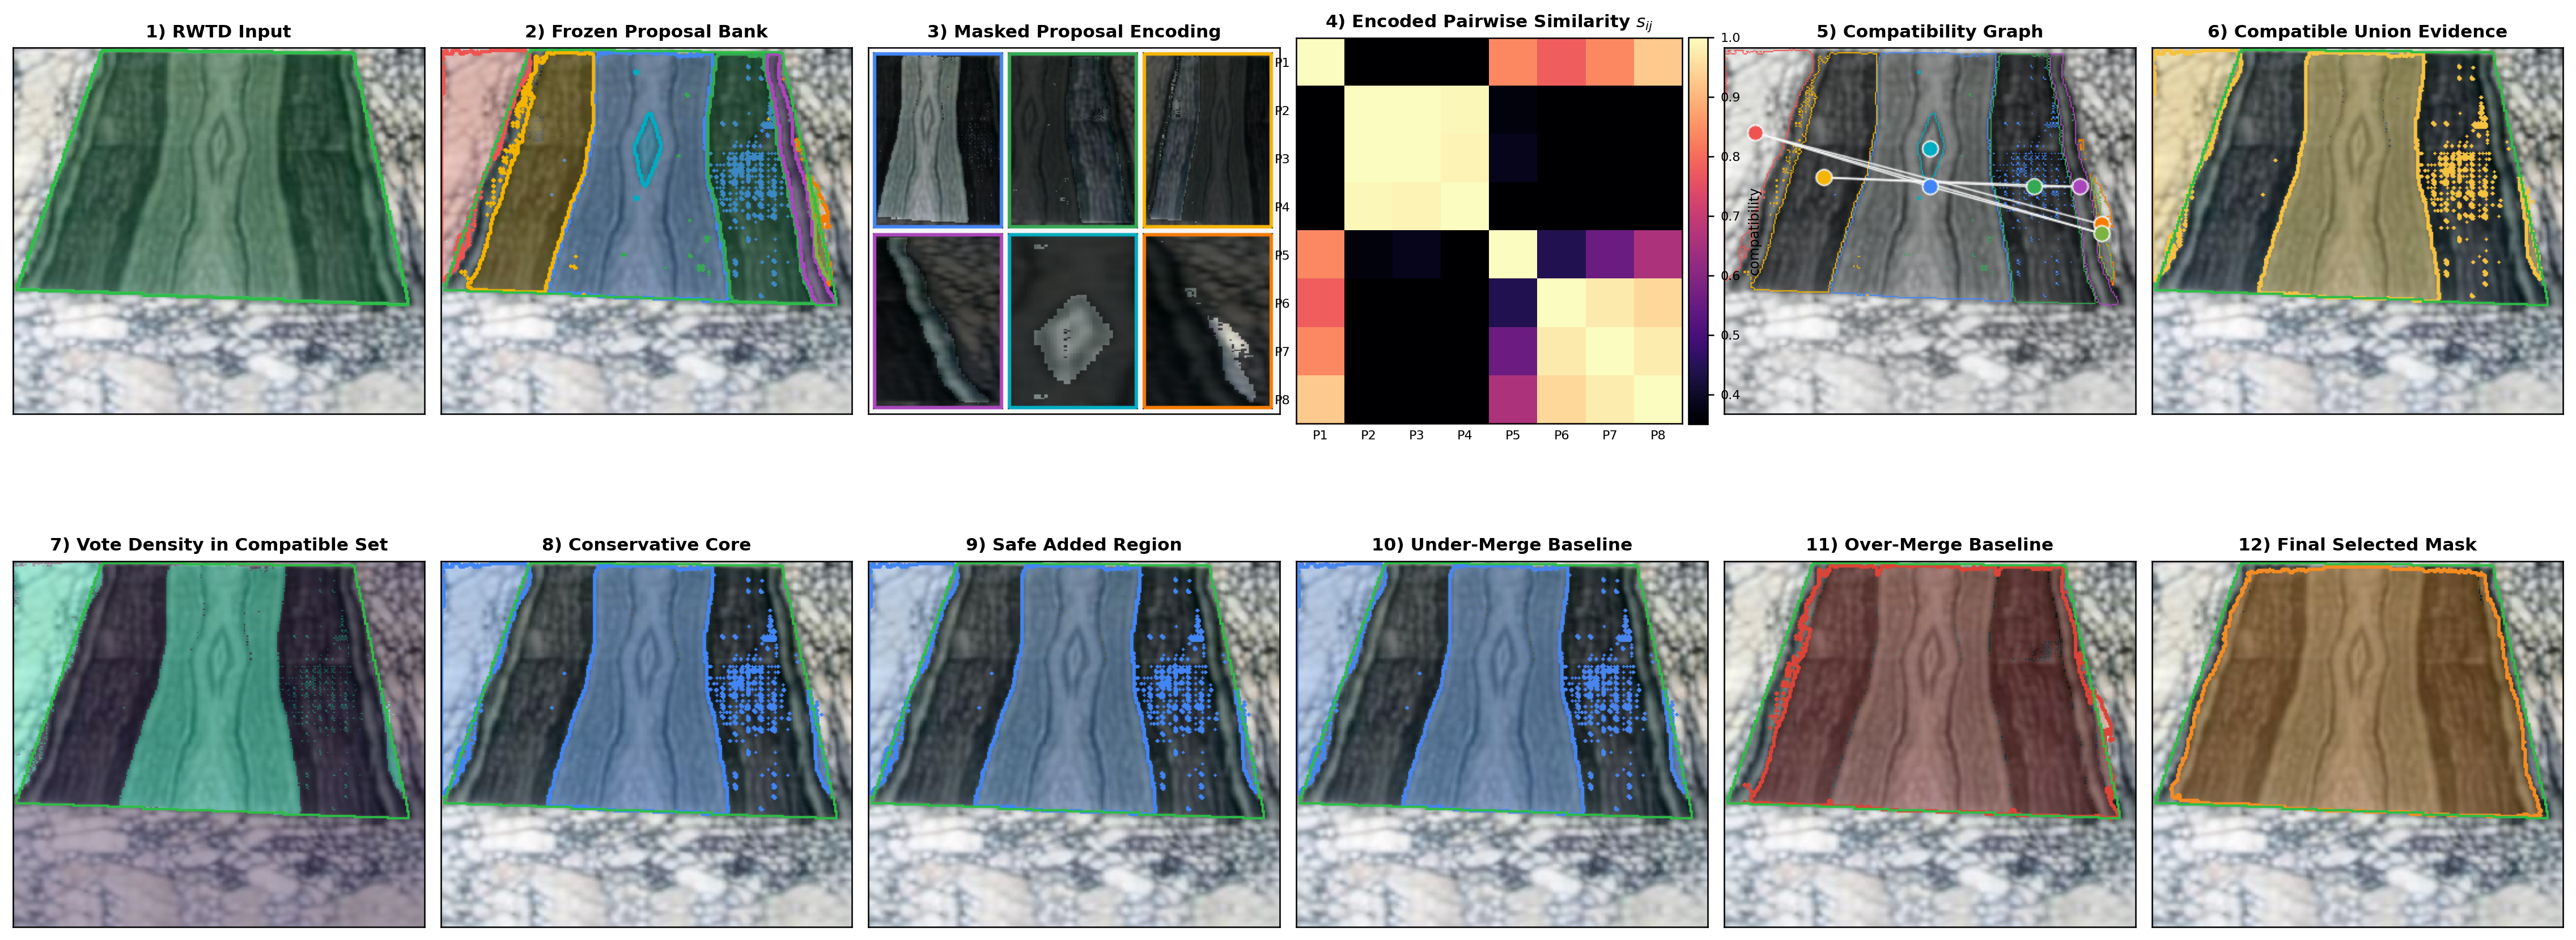
\includegraphics[width=0.98\textwidth]{figures/fig_consolidation_logic.png}
    \caption{Proposal-/mask-space exploration in implementation form. Each frozen proposal $m_i$ is encoded as a hybrid texture descriptor $d_i$, a learned pair model merges compatible proposals into candidate components, a learned component scorer selects a conservative core $C^\star$, and on RWTD only a learned dense-rescue switch can replace $C^\star$ with a denser candidate. Relative to the feature-space route, this figure answers a different question: not what the frozen representation contains internally, but what can already be recovered from the generated mask bank itself.}
    \label{fig:proposal_logic}
\end{figure*}

The implementation makes the learned objects explicit. Each proposal $m_i$ is encoded by a hybrid descriptor
\begin{align}
d_i = [h_i ; e_i],
\end{align}
where $h_i$ is a 60-D handcrafted summary of a 15-channel training-free texture map and $e_i$ is a PTD descriptor built from a masked crop plus ring context. The PTD encoder produces a 512-D region embedding, a second 512-D ring-context contrast term, and concatenates them into a 1024-D descriptor. The handcrafted map concatenates LAB color, Sobel $x/y/\|\nabla\|$, a Laplacian response, and an 8-filter Gabor bank; $h_i$ stores the mean, standard deviation, lower quartile, and upper quartile of those channels inside the proposal mask. Stage-A therefore uses a 1084-D descriptor per proposal.

Proposal compatibility is learned with a \textsc{RandomForestClassifier} over a 10-D pair feature vector. That vector includes descriptor cosine similarity, proposal area ratios, pair IoU, near-contact statistics, weak-boundary evidence, texture heterogeneity of the union, centroid distance, and union area ratio. Positive pair labels come from PTD-synthetic compositions: two proposals are compatible only when they cover the same synthetic texture region with sufficient purity. Thresholding these pair scores produces a compatibility graph, and its connected components define the candidate merged regions.

Candidate components are then ranked by a \textsc{RandomForestRegressor} over a second 10-D feature vector. Those component features include region area ratio, inside-versus-outside texture contrast, within-region variance, fragmentation penalty, boundary strength, compactness, descriptor variance within the component, descriptor separation from the complement, and proposal-count statistics. The regressor is trained to predict candidate IoU against the synthetic ground-truth partition, and the highest-scoring candidate becomes the conservative core $C^\star$.

RWTD adds one more learned decision layer above that core. A denser auxiliary bank proposes rescue candidates $R_k$ around under-covered scenes. For each $(C^\star, R_k)$ pair, the RWTD rescue path builds a core-versus-candidate feature vector that includes predicted score gaps, relative area and overlap, proposal-union coverage and precision, texture contrast, variance, and fragmentation deltas. A balanced logistic classifier predicts whether switching to $R_k$ is a safe positive move under \texttt{oracle\_safe\_winner} labels, and a \textsc{HistGradientBoostingRegressor} predicts the expected gain. The deployed \texttt{candidate\_cls} rule keeps the core unless some rescue candidate is classified positive, in which case it selects the positive candidate with highest predicted gain. STLD and the appendix routes stop at Stage-A and never invoke this rescue layer.
In notation,
\begin{align}
p_{\mathrm{safe}}(k) &= f_{\mathrm{safe}}(u(C^\star, R_k)),\\
g_{\mathrm{gain}}(k) &= f_{\mathrm{gain}}(u(C^\star, R_k)),
\end{align}
where $u(C^\star, R_k)$ is the rescue feature vector. The deployed prediction is
\begin{align}
\hat{Y}_{\mathrm{prop}} =
\begin{cases}
R_{k^\star}, & \exists k : p_{\mathrm{safe}}(k) > \tau_{\mathrm{safe}}, \; k^\star = \arg\max_{k: p_{\mathrm{safe}}(k) > \tau_{\mathrm{safe}}} g_{\mathrm{gain}}(k),\\
C^\star, & \text{otherwise.}
\end{cases}
\end{align}

\paragraph{Training regime and frozen components.} The proposal generator is frozen. This route does not retrain SAM, alter the prompt source, or optimize the bank with RWTD labels. What is learned instead is the decision stack above the bank. The RWTD Stage-A bundle used here is trained on 480 PTD-only synthetic samples, and the RWTD rescue bundle is trained on 256 PTD-only \texttt{repair\_mix} samples that inject explicit under-coverage cores and hard wrong-side decoys. The STLD Stage-A bundle is trained on 1600 PTD-only MPEG7-shape synthetic layouts. This separation is why the route speaks directly to recoverability: it measures how much task value remains once proposal generation is treated as fixed evidence rather than as the object of adaptation.

\paragraph{Why this model family?} The readout is deliberately small. The goal of the paper is to inspect what the frozen mask bank already contains, not to bury that question inside a new end-to-end network. The available supervision is limited and synthetic, the proposal descriptors mix heterogeneous geometric and texture cues, and the RWTD rescue path must remain modular enough to turn on only where it is needed. Tree-based models fit that regime well: they combine mixed tabular signals robustly, remain easy to audit at the level of pair scores and candidate rankings, and let the proposal bank stay fixed throughout. Appendix~\ref{app:implementation_details} summarizes the deployed inference algorithm, descriptor ablations, and the resulting practicality profile.

\section{Benchmarks and Evaluation Protocol}
\label{sec:data}

The paper's main scope is intentionally narrow. RWTD is the main natural benchmark and remains evaluation-only. STLD is the controlled synthetic companion with a canonical foreground side. Two additional routes remain in the appendix: a ControlNet-stitched bridge benchmark with exact binary supervision and a CAID breadth check. Neither route drives the main claim.

\paragraph{RWTD.} RWTD is the paper's anchor benchmark because it concentrates the failure modes that motivate recoverability: weak transitions, disconnected same-texture regions, and repeated-pattern distractors. Main results use the official evaluator plus a matched shared subset for direct comparison to the public TextureSAM rerun.

\paragraph{STLD.} STLD is the main synthetic companion. It is useful here because the shaped foreground side is canonical and exact supervision is available. That makes it a cleaner test of what the generated mask bank already reveals when evaluator ambiguity is minimal.

\paragraph{Supporting routes.} The appendix keeps two scope-limited routes. The ControlNet bridge benchmark is a controlled binary partition route generated by a ControlNet-conditioned stitched-regeneration pipeline; it preserves exact labels but uses more naturalistic transitions than classical hard mosaics. We use it as supporting evidence rather than a headline pillar because this paper does not establish a causal bridge-training effect. CAID is included as a domain-shift breadth check because its shoreline focus is less central to the paper's texture claim.

\paragraph{Metrics and subset conventions.} RWTD uses official mIoU and ARI under complementary binary partitions. STLD uses direct foreground mIoU and ARI because the shaped foreground side is canonical. The appendix bridge and CAID routes use partition-invariant mIoU and ARI. Every headline table keeps evaluator and subset conventions fixed within each comparison block; unmatched legacy numbers are not mixed into the main results.

\section{Results}
\label{sec:results}

We now use the two routes together to answer the central question. The feature-space route asks what frozen SAM reveals before any proposal reasoning. The proposal-/mask-space route asks what can already be recovered from the generated mask bank under matched benchmark protocols. Read together, they separate latent organization in the representation from recoverable organization in the generated masks.

\subsection{What does the feature-space route reveal?}

Feature-space exploration gives a cautious positive answer to \textbf{RQ1} and a direct answer to \textbf{RQ2}. Appendix~\ref{app:feature_provenance} shows that a clustering-only probe over pooled coarse \texttt{backbone\_fpn} features recovers plausible texture partitions, that coarse scale dominates finer native-grid controls, and that positional debiasing such as flip-averaging materially changes what is recovered. Read under its archived probe protocol rather than as a leaderboard comparison, the feature route shows that frozen features already organize texture-relevant structure.

This route is informative precisely because the readout is so light. No decoder is trained and no proposal reasoning is required. When pooled coarse features already separate repeated-pattern regions, transition cases, and shape-versus-texture examples, it becomes hard to argue that frozen SAM is entirely texture-blind. What the feature route does not settle by itself is how much of that latent structure has already been externalized into the generated masks under matched benchmark evaluation.

\subsection{What does the proposal-/mask-space route reveal?}

\begin{table*}[t]
\centering
\scriptsize
\setlength{\tabcolsep}{5pt}
\renewcommand{\arraystretch}{0.98}
\begin{tabularx}{\textwidth}{@{}p{0.16\textwidth}p{0.28\textwidth}Xcc@{}}
\toprule
Benchmark & Evaluator / subset & Method & mIoU & ARI \\
\midrule
RWTD & official invariant, full-256 & SAM2.1-small original rerun~\cite{ravi2024sam2} & 0.1615 & 0.2183 \\
RWTD & official invariant, full-256 & \sys{} final & 0.4611 & 0.6966 \\
RWTD & official invariant, common-253 & TextureSAM public checkpoint rerun~\cite{texturesamrepo2026} & 0.4684 & 0.6163 \\
RWTD & official invariant, common-253 & \sys{} final & 0.4645 & 0.7013 \\
\midrule
STLD & direct foreground, all-200 & SAM2.1-small original rerun~\cite{ravi2024sam2} & 0.3686 & 0.5269 \\
STLD & direct foreground, all-200 & \sys{} final & 0.6705 & 0.7249 \\
STLD & direct foreground, common-182 & TextureSAM public checkpoint rerun~\cite{texturesamrepo2026} & 0.5140 & 0.7526 \\
STLD & direct foreground, common-182 & \sys{} final & 0.7195 & 0.7791 \\
\bottomrule
\end{tabularx}
\caption{Main matched comparisons. Each block fixes the evaluator and subset convention before comparing methods. Supporting bridge and CAID routes are reported separately in the appendix so that the headline table remains protocol-matched.}
\label{tab:proposal_results}
\end{table*}


Proposal-/mask-space exploration answers the complementary question. On RWTD, the raw SAM2.1-small baseline is far below either texture-specialized adaptation or a lightweight readout above the frozen mask bank. Against the matched TextureSAM rerun on the shared RWTD subset, the proposal route reaches comparable overlap quality while improving partition coherence from 0.6163 to 0.7013 ARI. Because the official RWTD no-aggregation metric averages matched GT instances rather than simple per-image scores, we summarize uncertainty on the same overlap-instance view used by the paired analysis: the ARI gain is $+0.0995$ with a 95\% paired bootstrap interval of [$0.0721$, $0.1270$], while mIoU changes by $+0.0405$ [$0.0031$, $0.0764$]. The full official evaluator supports the same reading: the proposal route remains far above the raw SAM baseline at 0.4611 mIoU / 0.6966 ARI.

STLD shows the same route under cleaner synthetic geometry. On the matched shared subset, the proposal route improves from 0.5140 / 0.7526 to 0.7195 / 0.7791, and paired per-image bootstraps remain positive on average across both the matched subset and all-image view. The ARI gain is smaller than the RWTD gain, but it remains directionally consistent with the claim that generated masks contain recoverable texture structure. Together, RWTD and STLD show that substantial texture task value can be recovered from the frozen mask bank without retraining the backbone or proposal generator.

Appendix~\ref{app:implementation_details} shows that this result is not reducible to one lucky descriptor stack and also reports the practicality profile of the readout. The hybrid descriptor helps most on the harder fragmented RWTD regime, but the proposal-route claim survives across descriptor families, and the measured runtime remains modest for a lightweight layer above a fixed bank.

\subsection{What do the two routes reveal together?}

The two routes are parallel in question but different in what they expose. Feature-space exploration reveals latent organization in the frozen representation before any explicit mask reasoning. Proposal-/mask-space exploration reveals whether that organization has already been externalized into the generated masks strongly enough to recover a coherent texture partition. The first route is therefore most informative about existence and localization of texture-relevant structure; the second is most informative about recoverability under matched end-task evaluation.

\begin{figure*}[t]
    \centering
    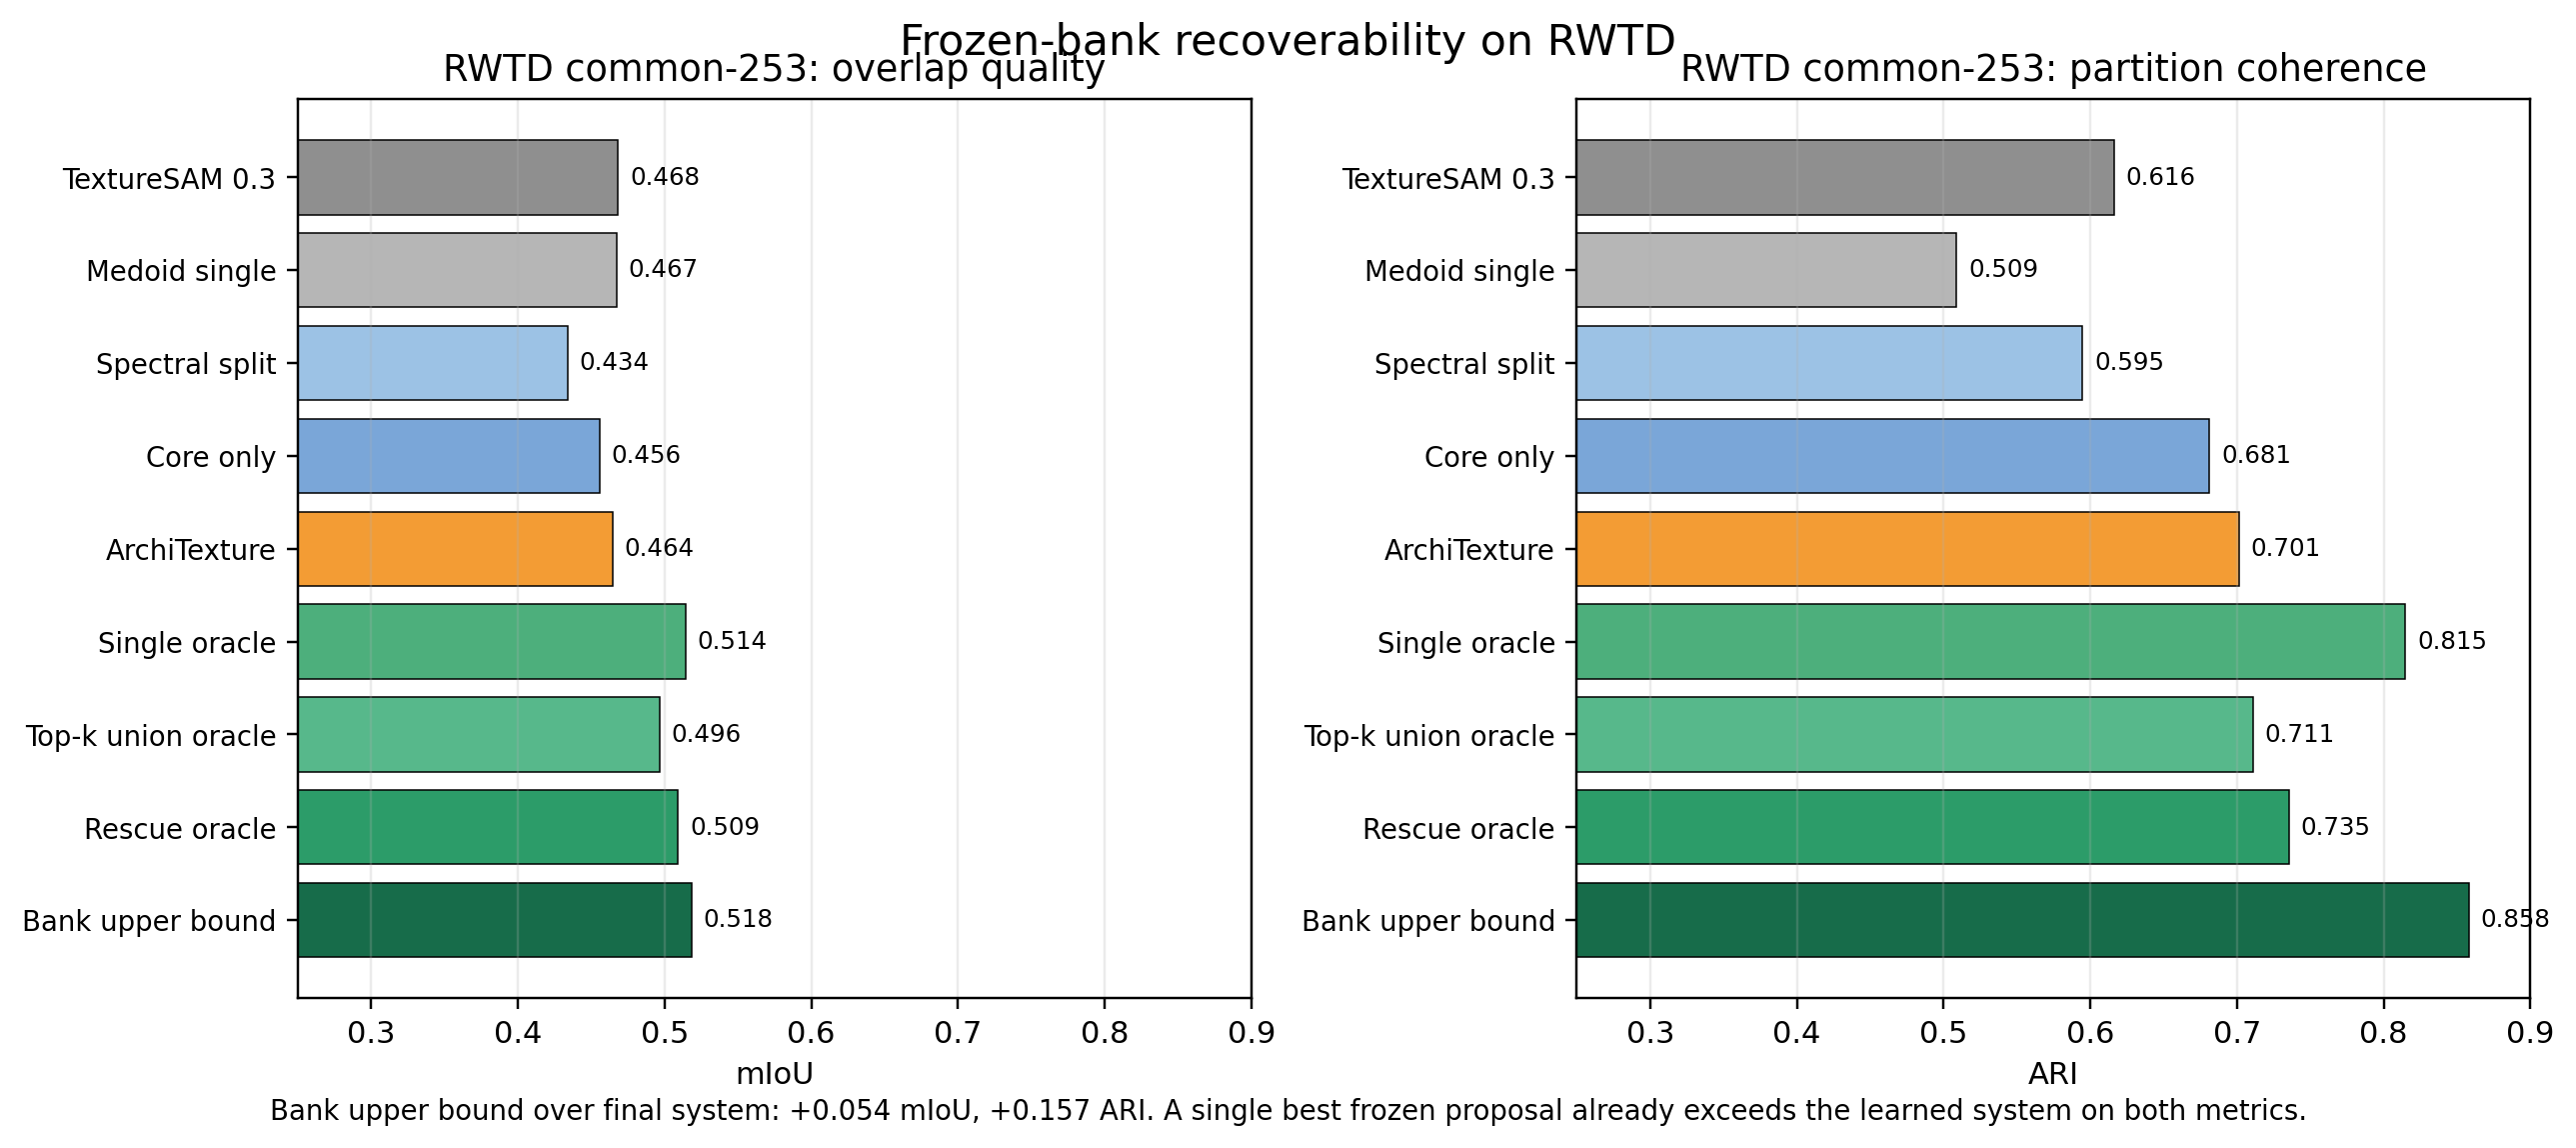
\includegraphics[width=0.98\textwidth]{figures/fig_rwtd_oracle_decomposition.png}
    \caption{Proposal-/mask-space route on RWTD. Generic frozen-bank heuristics are noticeably weaker than the learned readout, but the bank oracles remain substantially higher still. The figure therefore makes the route-specific message concrete: generated masks on natural fragmented scenes already contain substantial texture evidence, but that evidence is often distributed across fragments and low-margin alternatives.}
    \label{fig:rwtd_oracle_decomp}
\end{figure*}

\begin{table}[t]
\centering
\scriptsize
\begin{tabular}{@{}lcc@{}}
\toprule
RWTD common-253 method & mIoU & ARI \\
\midrule
Medoid single & 0.4673 & 0.5087 \\
Learned single selector & 0.4512 & 0.5601 \\
Spectral split & 0.4339 & 0.5948 \\
Agglomerative split & 0.4354 & 0.5898 \\
Greedy merge & 0.4442 & 0.5197 \\
Core only & 0.4558 & 0.6812 \\
\sys{} final & 0.4645 & 0.7013 \\
Single frozen-proposal oracle & 0.5142 & 0.8146 \\
Top-$k$ union oracle & 0.4964 & 0.7107 \\
Rescue candidate oracle & 0.5093 & 0.7352 \\
Bank upper bound & 0.5183 & 0.8580 \\
\bottomrule
\end{tabular}
\caption{RWTD recoverability decomposition on the matched common-253 subset. The learned top-1 selector is stronger than the medoid single baseline, but it still trails the full commitment stack by a wide ARI margin. The bank oracles remain far higher still. The omitted compatible-component oracle performs poorly (0.4748 mIoU / 0.2497 ARI), which is evidence that compatibility merging alone is not sufficient.}
\label{tab:oracle_recoverability}
\end{table}


RWTD makes \textbf{RQ4} concrete. A single frozen proposal can already be very strong, and the bank upper bound is higher still. Yet learned top-1 selection still trails the full readout by a wide ARI margin. The generated masks therefore contain substantial texture structure, but that structure is often distributed across multiple fragments or low-margin alternatives. This is where the proposal route reveals something the feature route cannot: the representation may already be organized, but the generated masks still need commitment to turn that organization into the right partition.

STLD gives the complementary answer. There, a learned single-proposal selector already nearly matches the full readout, which means the generated masks often already contain a coherent singleton answer. \Cref{tab:stld_selector_contrast} captures the regime contrast directly: RWTD is primarily a fragmented-evidence problem, while STLD is often a singleton-selection problem. Seen alongside the feature route, this contrast clarifies the joint interpretation. Frozen features expose texture organization broadly, while the generated masks determine whether that organization appears as fragmented evidence requiring commitment or as a nearly complete mask already available for selection.

\begin{table*}[t]
\centering
\scriptsize
\setlength{\tabcolsep}{5pt}
\renewcommand{\arraystretch}{0.98}
\begin{tabularx}{\textwidth}{@{}p{0.22\textwidth}Xcc@{}}
\toprule
Route & Variant & mIoU & ARI \\
\midrule
RWTD common-253 & Medoid single (generic bank baseline) & 0.4673 & 0.5087 \\
RWTD common-253 & Learned single selector & 0.4512 & 0.5601 \\
RWTD common-253 & Conservative core only & 0.4558 & 0.6812 \\
RWTD common-253 & Proposal route final & 0.4645 & 0.7013 \\
\midrule
STLD common-182 & Proposal union & 0.2543 & 0.1731 \\
STLD common-182 & Handcrafted consolidation & 0.3680 & 0.3987 \\
STLD common-182 & PTD heuristic & 0.3757 & 0.4085 \\
STLD common-182 & Learned single selector & 0.7196 & 0.7731 \\
STLD common-182 & Proposal route final & 0.7195 & 0.7791 \\
\midrule
ControlNet bridge all-1742 & Proposal union (synthetic complement) & 0.6749 & 0.1188 \\
ControlNet bridge all-1742 & Proposal route Stage-A (synthetic complement) & 0.6803 & 0.6039 \\
\bottomrule
\end{tabularx}
\caption{Route-specific evidence for \textbf{RQ4} using each route's native evaluator. On RWTD, learned top-1 selection helps but remains well below the structured commitment stack, while the conservative core already captures most of the coherence gain and the final rescue layer adds the remaining improvement. On STLD, by contrast, learned top-1 selection is already very strong, which highlights the difference between canonical synthetic partitions and the more fragmented natural RWTD scenes. The ControlNet bridge rows show that a simple proposal union remains inadequate even on the broader synthetic complement.}
\label{tab:proposal_ablation}
\end{table*}


Seen together, the routes suggest a simple joint interpretation. Frozen SAM is not missing texture structure altogether: the feature route reveals it internally, and the proposal route reveals that much of it has already been externalized into the generated mask bank. Their difference is where the unresolved difficulty lies. Features show that the representation is textured enough to support meaningful clustering; masks show that on natural fragmented scenes the remaining failure is commitment among partially correct proposals rather than total absence of relevant evidence.

\subsection{What remains unrecovered?}

The paper's answer is therefore incomplete in a precise way. Neither route fully closes ambiguity. The feature route can reveal latent organization, but it does not settle the final partition choice under matched benchmark evaluation. The proposal route can recover strong partitions, but the remaining oracle gap shows that the unresolved issue is less whether the mask bank ever contains the answer than whether the readout preserves multiple plausible hypotheses long enough to choose correctly. Appendix~\ref{app:rwtd_diag} expands this point with selector/core/final/oracle case studies, and Appendix~\ref{app:stld_support} shows the complementary STLD regime where a coherent singleton often already exists.

\section{Discussion and Limitations}
\label{sec:discussion}

The paper's central question was whether frozen SAM contains texture understanding despite not being built as a texture segmenter. The answer is yes, but only in the sense of \emph{recoverable} texture-relevant structure. The paper does not show that frozen SAM already outputs the right texture partition by default. It shows instead that frozen SAM contains more texture-relevant evidence than its raw outputs reveal.

\paragraph{What we learn from frozen features.} Feature-space exploration answers the existence question positively but cautiously. Coarse frozen features are not texture-blind: they already support nontrivial binary texture partitions under a clustering-only readout. That matters because it shows that the frozen backbone already contains texture-relevant organization before any learned decoder or proposal reasoning.

\paragraph{What we learn from generated masks.} Proposal-/mask-space exploration shows that the generated mask bank also contains substantial texture-relevant structure. On matched RWTD and STLD evaluations, a lightweight readout above frozen proposals recovers strong texture partitions without retraining the proposal generator. The generated masks are therefore not merely noisy by-products; they often already externalize useful texture evidence.

\paragraph{What the two routes jointly imply.} Read together, the routes argue against a simple ``frozen SAM is texture-blind'' conclusion. Frozen SAM carries texture-relevant structure internally and often exposes enough of it in its generated masks to support strong downstream partitions. The difference between the routes is not importance but stage of inspection: features reveal latent organization, while generated masks reveal recoverable partition structure.

\paragraph{Where the routes differ.} The routes are conceptually parallel but empirically asymmetric. The feature probe is reported under an archived probe protocol, so it is most informative about existence and organization of texture structure. The proposal route supports the matched benchmark comparisons and therefore says more about end-task recoverability. Across datasets, RWTD shows fragmented mask evidence that benefits from structured commitment, while STLD often already contains a coherent singleton mask. This is a difference in what the generated masks reveal, not a reason to dismiss either route.

\paragraph{What remains unresolved.} The remaining limitation is not mainly proposal absence. It is ambiguity handling above a strong bank. The current proposal route still makes low-margin wrong-partition commitments on RWTD, and the oracle gap shows that preserving multiple plausible hypotheses for longer could close further headroom. The feature route remains tied to its archived probe protocol, the appendix bridge route does not establish a causal bridge-training benefit, and CAID remains a breadth check rather than a central texture benchmark. The next step is therefore not necessarily a different frozen backbone. It is better uncertainty-aware commitment above fragmented generated masks: calibration, abstention, or multi-hypothesis outputs that avoid premature collapse to the wrong partition.

\section{Reproducibility Note}
\label{sec:repro}

Every headline number is traceable to a rerun or a named artifact in \texttt{EXPERIMENT\_LEDGER.md} and \texttt{UPDATED\_SOURCES\_USED.md}. RWTD remains evaluation-only throughout the paper: no main claim depends on RWTD-label training or hyperparameter search. The manuscript workspace is self-contained, so paper compilation does not depend on older manuscript trees or external figure paths.


{\small
\bibliographystyle{plainnat}
\bibliography{refs}
}

\clearpage
\appendix
\section{Implementation Details and Practicality}
\label{app:implementation_details}

\begin{table}[t]
\centering
\footnotesize
\setlength{\tabcolsep}{0pt}
\renewcommand{\arraystretch}{1.02}
\begin{tabularx}{\columnwidth}{@{}X@{}}
\toprule
\textbf{Algorithm 1: \sys{} proposal-space inference for image $x$} \\
\midrule
1. Load the frozen prompt-bank proposals $\mathcal{P}(x)$ and compute proposal descriptors $d_i$ for each $m_i \in \mathcal{P}(x)$. \\
2. Score adjacent proposal pairs with $s(i,j)$ and threshold the compatibility graph. \\
3. Form candidate merged regions from the graph connected components. \\
4. Score each candidate with $q(C)$ and choose the conservative core $C^\star = \arg\max_C q(C)$. \\
5. If the route is RWTD, build dense rescue candidates $R_k$ from the auxiliary bank $\mathcal{P}^{+}(x)$. \\
6. Score each $(C^\star, R_k)$ with the safe-switch classifier $p_{\mathrm{safe}}(k)$ and gain regressor $g_{\mathrm{gain}}(k)$. \\
7. Output the positive rescue candidate with highest predicted gain, if any; otherwise output $C^\star$. \\
\bottomrule
\end{tabularx}
\caption{Compact pseudocode for the deployed decision layer. STLD and the appendix routes stop after Step~4 because they do not use the RWTD rescue layer.}
\label{tab:algorithm_box}
\end{table}

\begin{table*}[t]
\centering
\scriptsize
\setlength{\tabcolsep}{4pt}
\renewcommand{\arraystretch}{0.98}
\resizebox{\textwidth}{!}{%
\begin{tabular}{@{}llcccccc@{}}
\toprule
Benchmark / subset & Output & \multicolumn{2}{c}{Handcrafted-only} & \multicolumn{2}{c}{PTD-only} & \multicolumn{2}{c}{Hybrid} \\
 &  & mIoU & ARI & mIoU & ARI & mIoU & ARI \\
\midrule
RWTD common-253 & Stage-A official & 0.4469 & 0.6556 & 0.4486 & 0.6505 & 0.4558 & 0.6812 \\
RWTD full-256 & Stage-A official & 0.4454 & 0.6533 & 0.4472 & 0.6484 & 0.4543 & 0.6786 \\
STLD common-182 & Stage-A direct & 0.7045 & 0.7808 & 0.6698 & 0.7740 & 0.7195 & 0.7791 \\
STLD all-200 & Stage-A direct & 0.6570 & 0.7265 & 0.6253 & 0.7203 & 0.6705 & 0.7249 \\
\bottomrule
\end{tabular}
}
\caption{Descriptor ablation for the descriptor-sensitive Stage-A commitment layer, with the proposal bank, evaluator, and model family held fixed. RWTD is reported at Stage-A because the dense rescue layer operates on candidate masks and is unchanged across descriptor variants. Hybrid descriptors are clearly strongest on RWTD, while STLD is less sensitive to the descriptor choice and even slightly favors handcrafted-only on ARI.}
\label{tab:descriptor_ablation}
\end{table*}

\begin{table*}[t]
\centering
\scriptsize
\setlength{\tabcolsep}{3pt}
\renewcommand{\arraystretch}{0.98}
\begin{tabularx}{\textwidth}{@{}p{0.14\textwidth}ccccccX@{}}
\toprule
Route & Prompt props & Merged comps & Dense props & Rescue cand. & s / img & Peak RSS & Reading \\
\midrule
RWTD Stage-A & 3.84 & 2.64 & -- & -- & 0.025 & 430 MiB & prompt-bank commitment only \\
RWTD full & 3.84 & 2.64 & 38.05 & 11.72 & 0.378 & 637 MiB & dense rescue evaluated on the full set; 21/256 images switch \\
STLD Stage-A & 1.78 & 2.32 & -- & -- & -- & -- & no rescue path; no separate runtime profile recorded \\
\bottomrule
\end{tabularx}
\caption{Practicality profile of the deployed decision layer. RWTD timings come from measured full-dataset GPU profiles of the same frozen-bank pipeline. STLD shares the same Stage-A architecture and bank statistics, but no separate runtime profile was recorded in the repository.}
\label{tab:practicality}
\end{table*}


\paragraph{Why include this appendix section?} The paper's main claim is scientific rather than systems-oriented, but two reviewer questions still matter: whether the gain depends mainly on a particular descriptor stack, and whether the decision layer is practical enough to deploy above a frozen bank. The tables in this section answer those questions directly. The descriptor ablation keeps the decision stack fixed while varying only the proposal descriptor in the descriptor-sensitive Stage-A layer; on RWTD, hybrid descriptors help clearly more than either single family, while STLD is noticeably less sensitive and sometimes slightly favors handcrafted cues on ARI. The practicality table then summarizes the actual bank sizes, rescue scale, and measured runtime profile of the deployed RWTD and STLD routes.

\section{Feature-Space Evidence}
\label{app:feature_provenance}

The feature-space route is reported under its archived probe protocol. Its repository-backed artifacts come from the coarse-feature clustering bundles, the parity summaries, and the scale-probe study in the \texttt{research-site} tree. The key caveat is short and fixed throughout this appendix: the RWTD feature probe does not use the official proposal-route evaluator, so this route is read as evidence for where texture structure can already live inside frozen features rather than merged into the matched proposal-route tables.

\begin{figure*}[t]
    \centering
    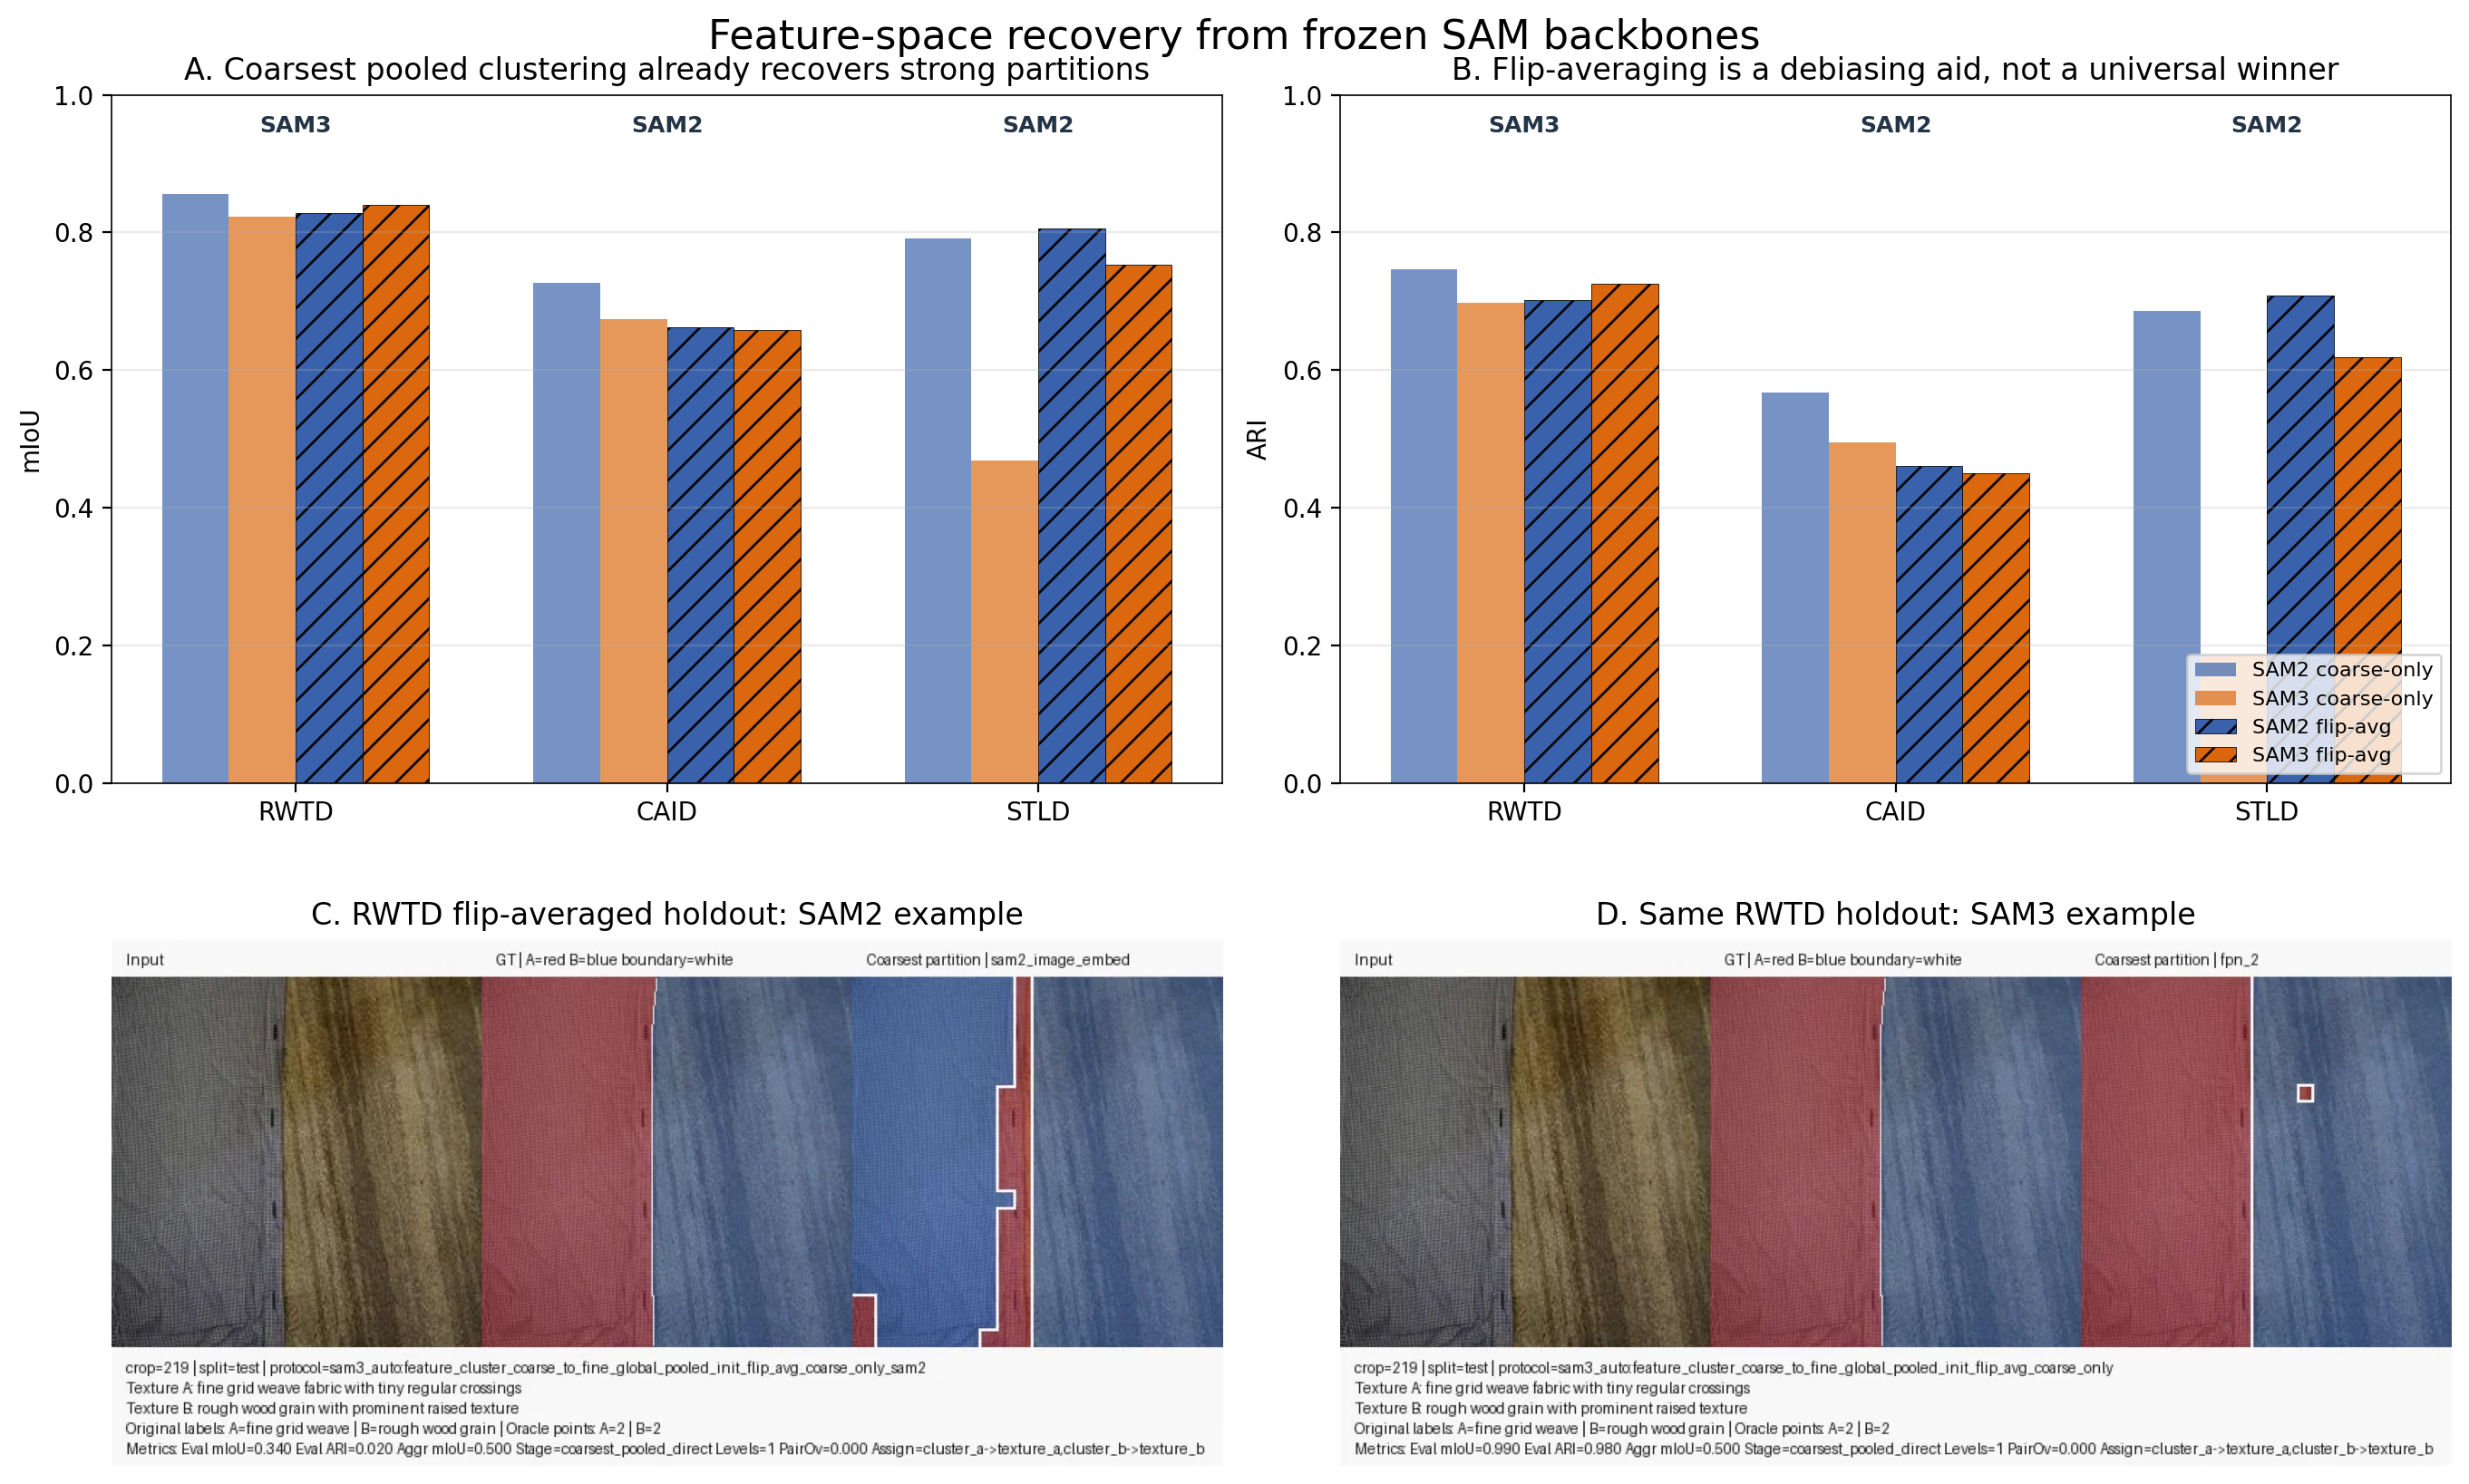
\includegraphics[width=0.98\textwidth]{figures/fig_feature_space_recovery.png}
    \caption{Archived feature-probe summary from the repository parity bundles. Top: coarse-only and flip-averaged summaries across RWTD, STLD, and CAID. Bottom: representative RWTD holdouts showing that coarse clustering can recover plausible binary partitions while remaining sensitive to positional bias.}
    \label{fig:feature_summary_app}
\end{figure*}

\begin{figure*}[t]
    \centering
    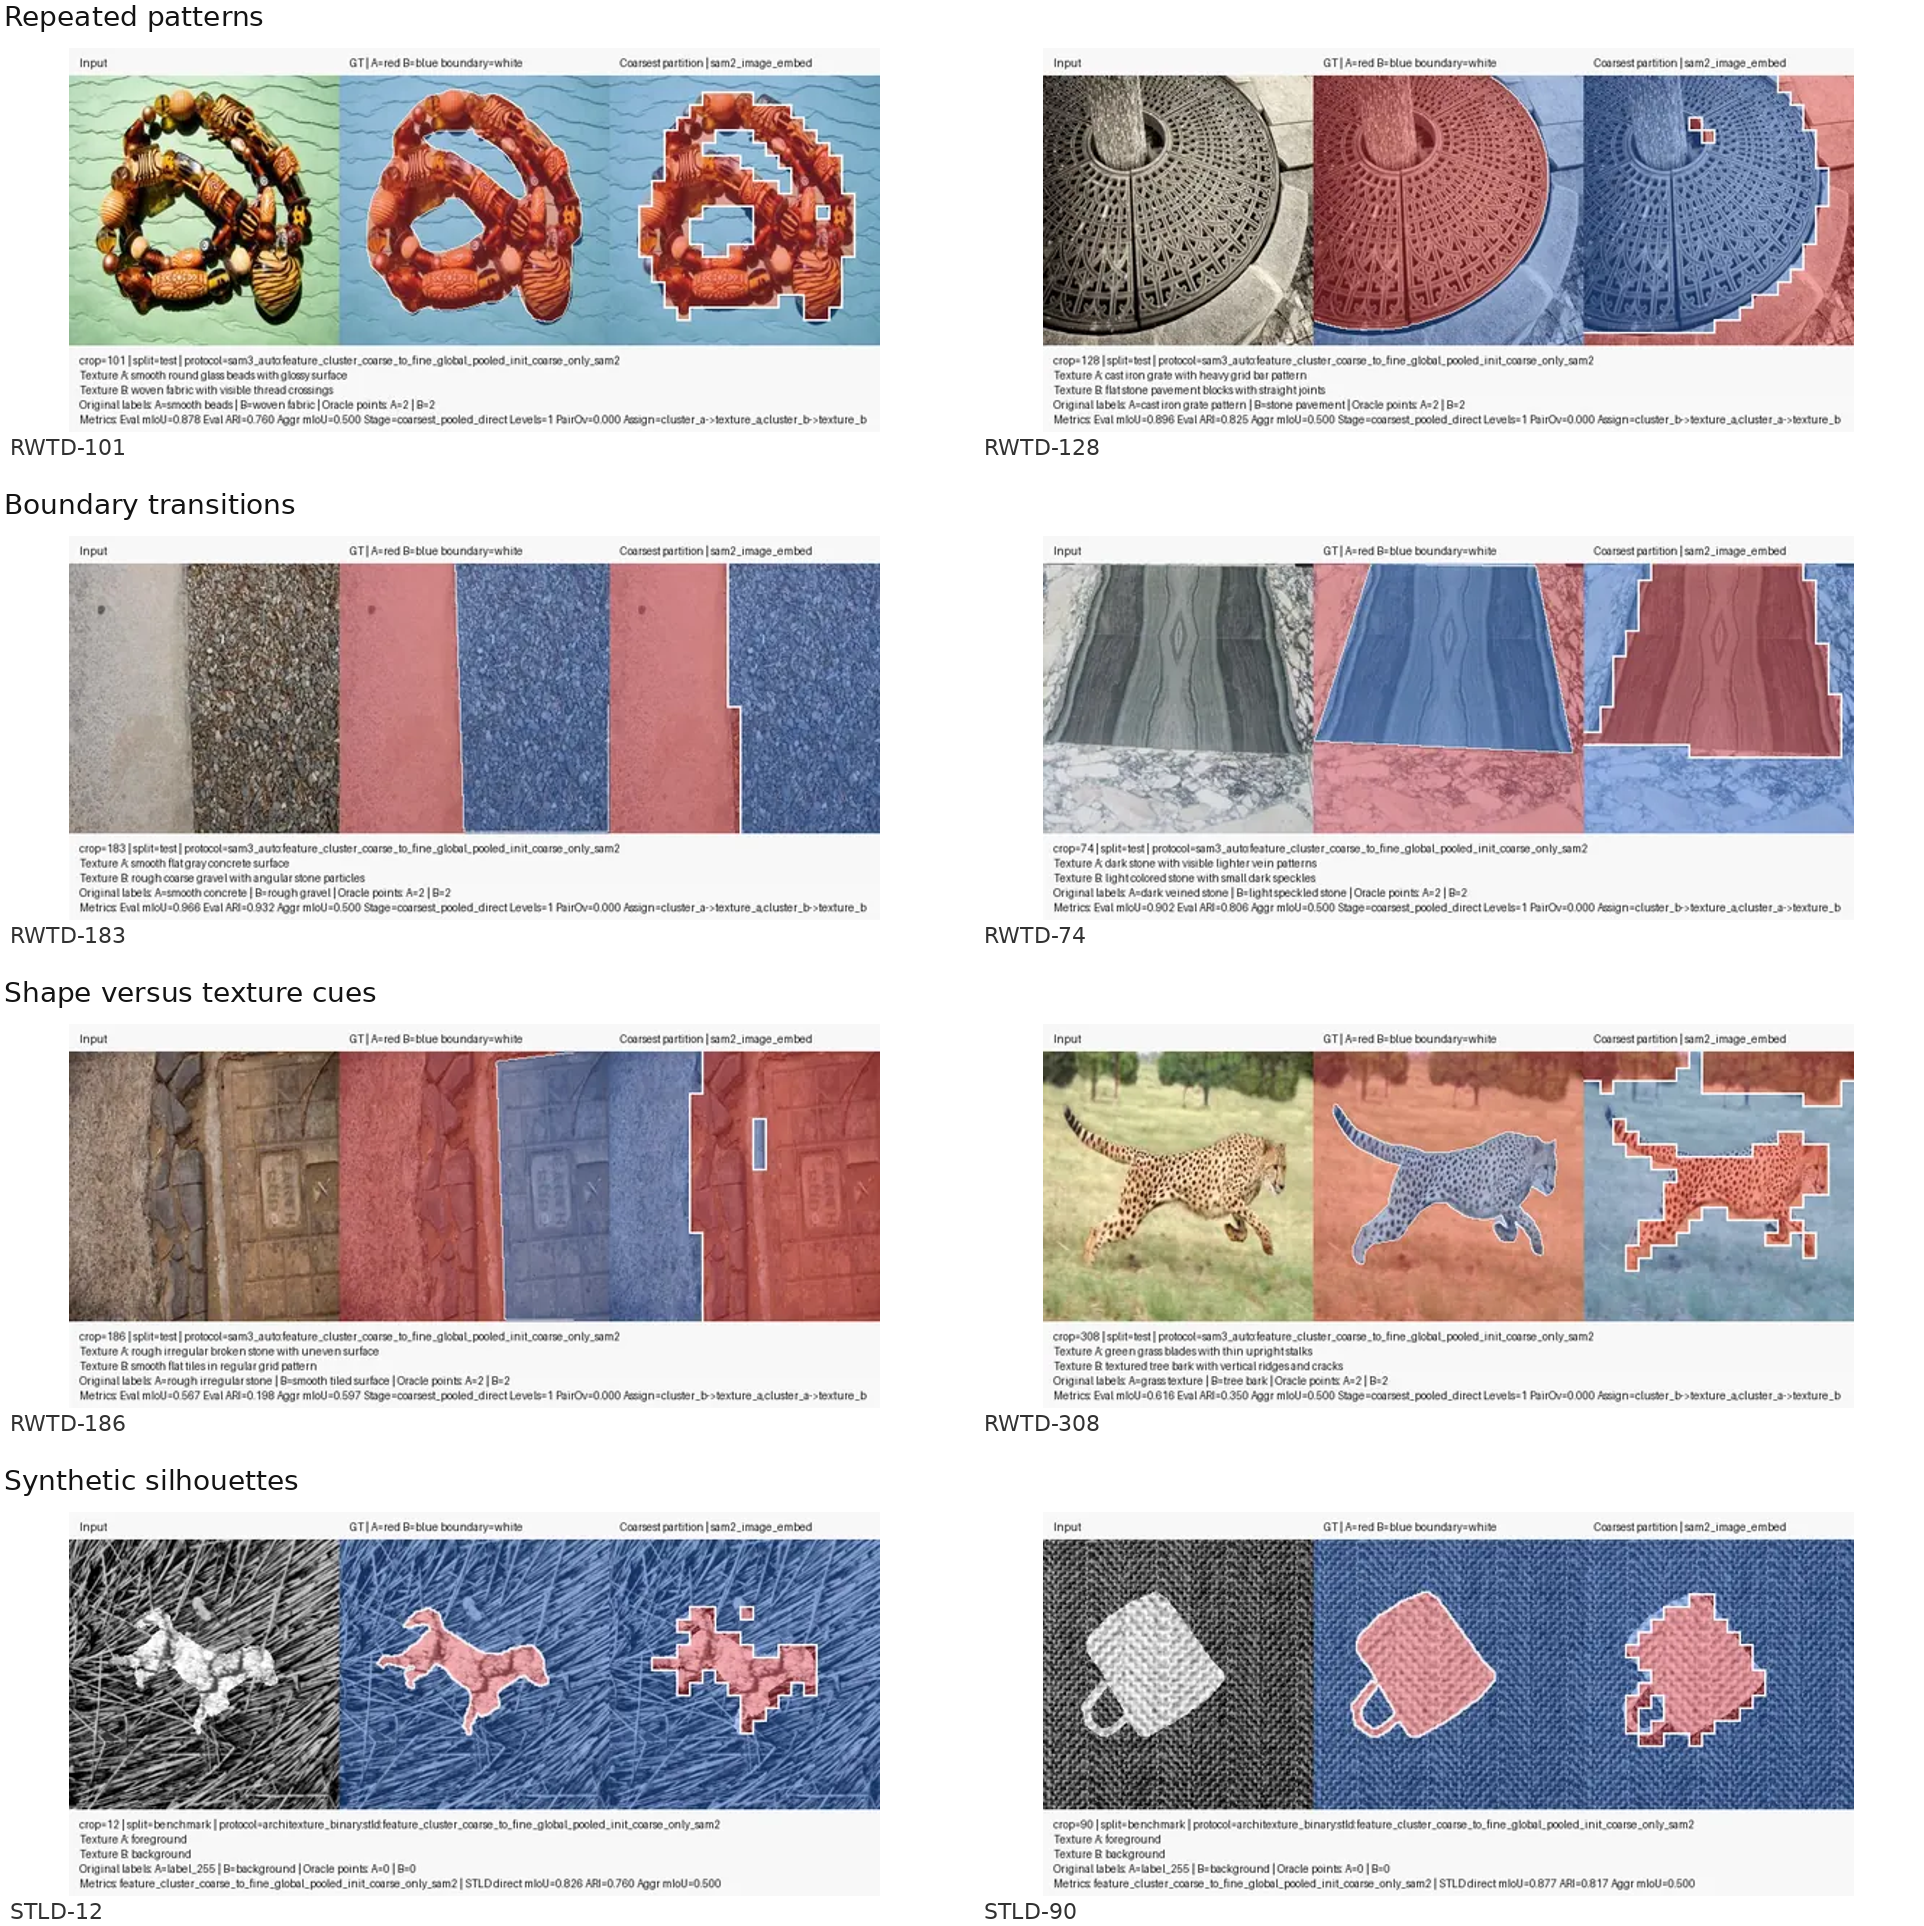
\includegraphics[width=0.98\textwidth]{figures/fig_feature_gallery.png}
    \caption{Curated qualitative gallery for coarse frozen-feature clustering. The gallery spans repeated-pattern scenes, gradual texture transitions, shape-versus-texture cases, and synthetic silhouettes. The annulus example in RWTD-101 is representative of the strongest qualitative evidence: even a frozen coarse probe can recover a topologically nontrivial partition without retraining the backbone.}
    \label{fig:feature_gallery}
\end{figure*}

\begin{figure*}[t]
    \centering
    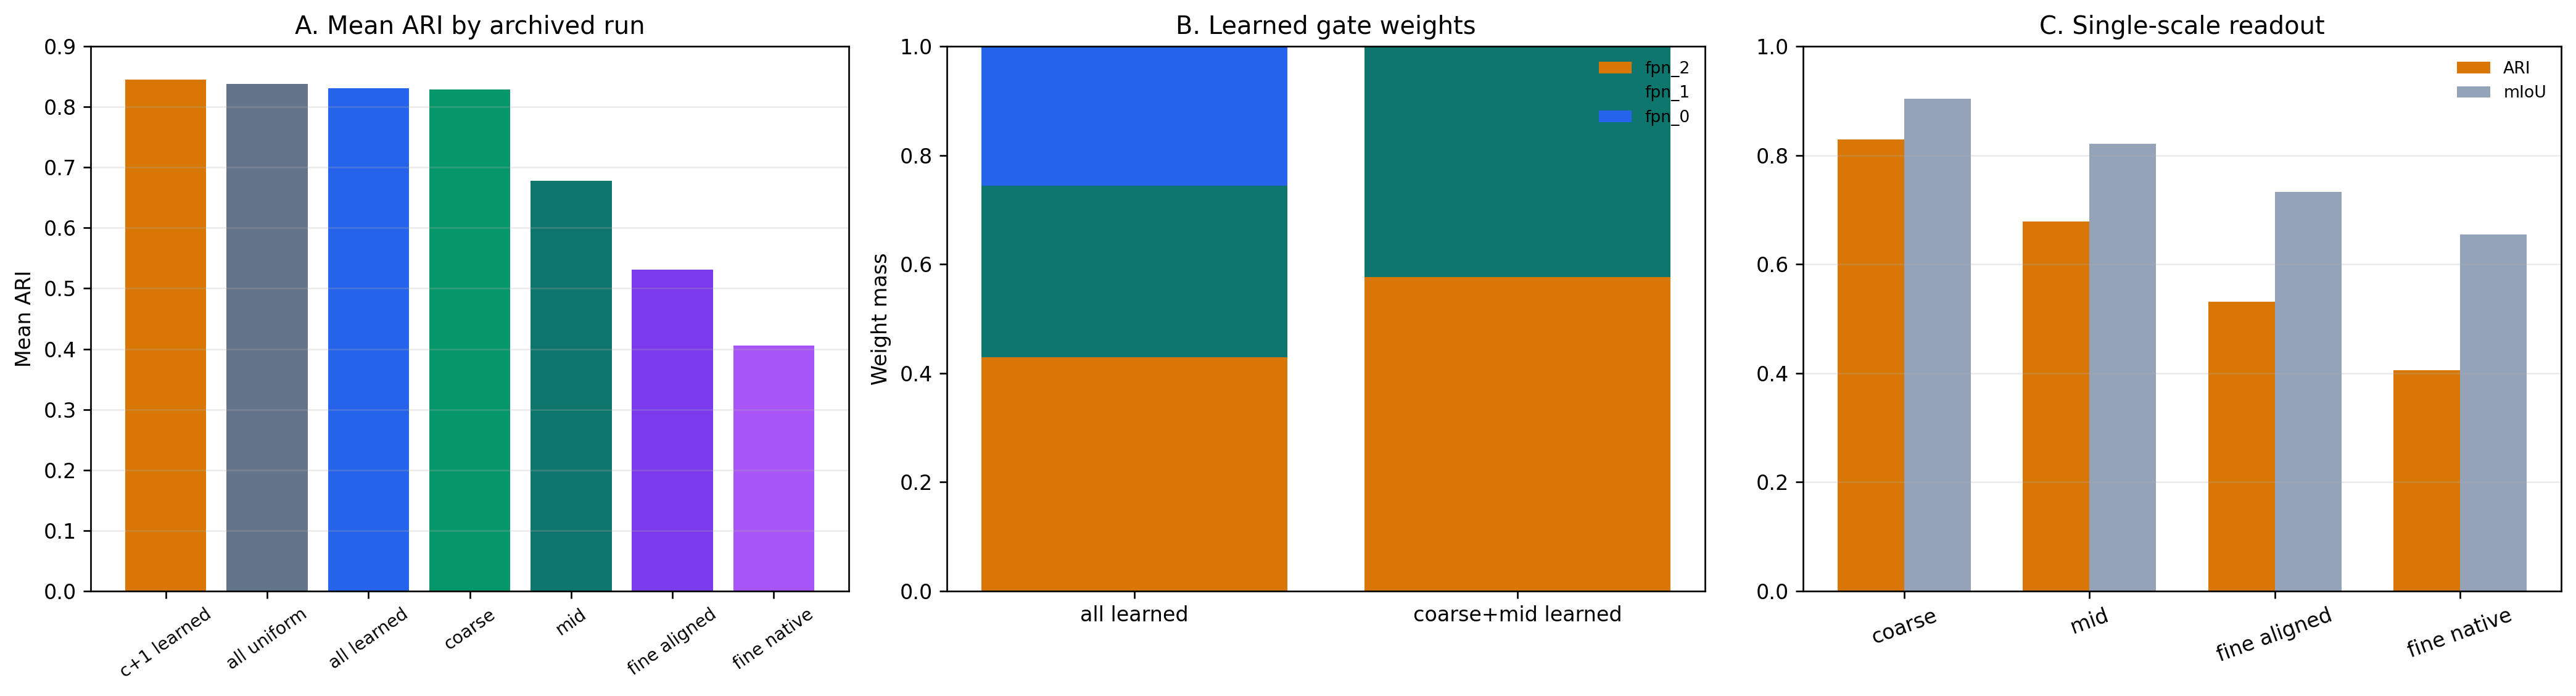
\includegraphics[width=0.98\textwidth]{figures/fig_feature_scale_diagnostics.png}
    \caption{Archived scale and gating diagnostics from the feature probe. Left: mean ARI by run. Middle: learned all-scale and coarse-plus-mid gate weights still place most mass on the coarsest level. Right: single-scale readouts show that coarse features dominate, while native fine-grid clustering is the weakest control. These runs are read as archived probe evidence rather than as matched benchmark comparisons.}
    \label{fig:feature_scale_diag}
\end{figure*}

\paragraph{Interpretation.} The appendix diagnostics point in one direction. Coarse frozen features already recover much of the binary partition on the repository-backed probe, learned all-scale fusion still prefers the coarsest level, and the finest native grid is the least reliable setting. That is enough for the paper's use of this route: frozen SAM features can contain texture-aware structure, even though the feature probe is not the matched benchmark route used for RWTD and STLD headline comparisons.

\begin{table}[t]
\centering
\scriptsize
\setlength{\tabcolsep}{4pt}
\renewcommand{\arraystretch}{0.98}
\resizebox{\columnwidth}{!}{%
\begin{tabular}{@{}llcccc@{}}
\toprule
Dataset & Eval view & SAM2 coarse-only & SAM3 coarse-only & SAM2 flip-avg & SAM3 flip-avg \\
\midrule
RWTD & partition-invariant & 0.8561 / 0.7472 & 0.8235 / 0.6984 & 0.8278 / 0.7013 & 0.8397 / 0.7258 \\
CAID & partition-invariant & 0.7263 / 0.5673 & 0.6743 / 0.4956 & 0.6620 / 0.4605 & 0.6588 / 0.4507 \\
STLD & direct foreground & 0.7908 / 0.6864 & 0.4682 / 0.1859 & 0.8064 / 0.7089 & 0.7534 / 0.6194 \\
\bottomrule
\end{tabular}
}
\caption{Archived frozen-feature parity summary from the site bundle. Each cell is reported as mIoU / ARI. This table is reported under the archived feature-probe protocol and is not merged into the matched proposal-route benchmark tables.}
\label{tab:feature_parity}
\end{table}


\section{RWTD Oracle and Failure Details}
\label{app:rwtd_diag}

RWTD is where the recoverability claim is most demanding. The proposal bank is strong, but the deployed decision stack still leaves a large oracle gap. \Cref{fig:rwtd_case_gallery} shows four recurring patterns. First, top-1 proposal scoring can miss cases where conservative component commitment succeeds. Second, rescue can repair an under-covered core. Third, a strong singleton can already exist in the bank even when the deployed stack abstains from it. Fourth, the remaining wrong-partition failures are low-margin commitment mistakes rather than proposal-bank misses.

\begin{figure*}[t]
    \centering
    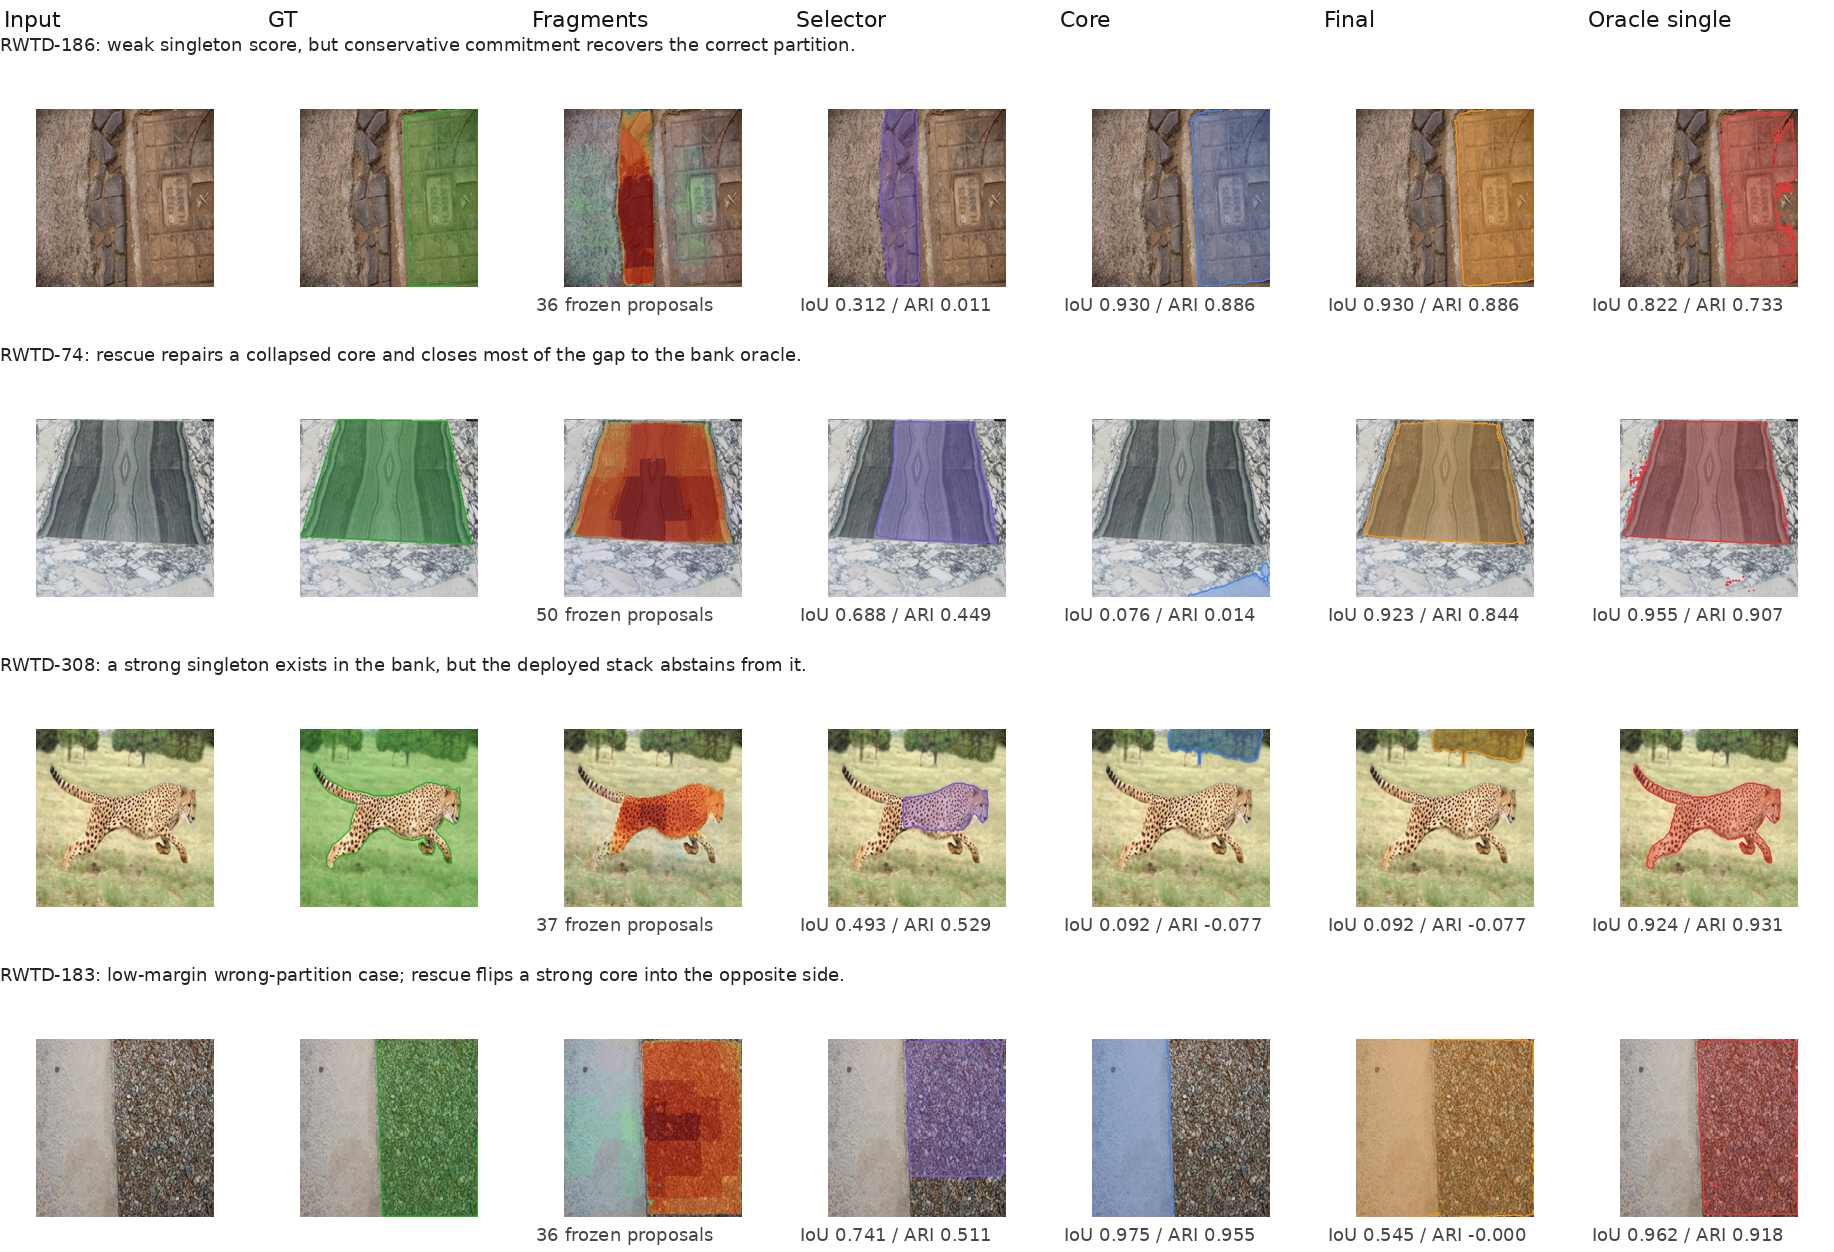
\includegraphics[width=\textwidth]{figures/fig_rwtd_case_gallery.png}
    \caption{RWTD case studies across selector, core, final, and oracle views. These examples make the oracle gap concrete: the bank often contains a strong answer, but the deployed stack still needs the right commitment decision to reach it. The rescue layer helps on some under-coverage cases, but low-margin wrong-partition failures remain brittle.}
    \label{fig:rwtd_case_gallery}
\end{figure*}

\begin{figure*}[t]
    \centering
    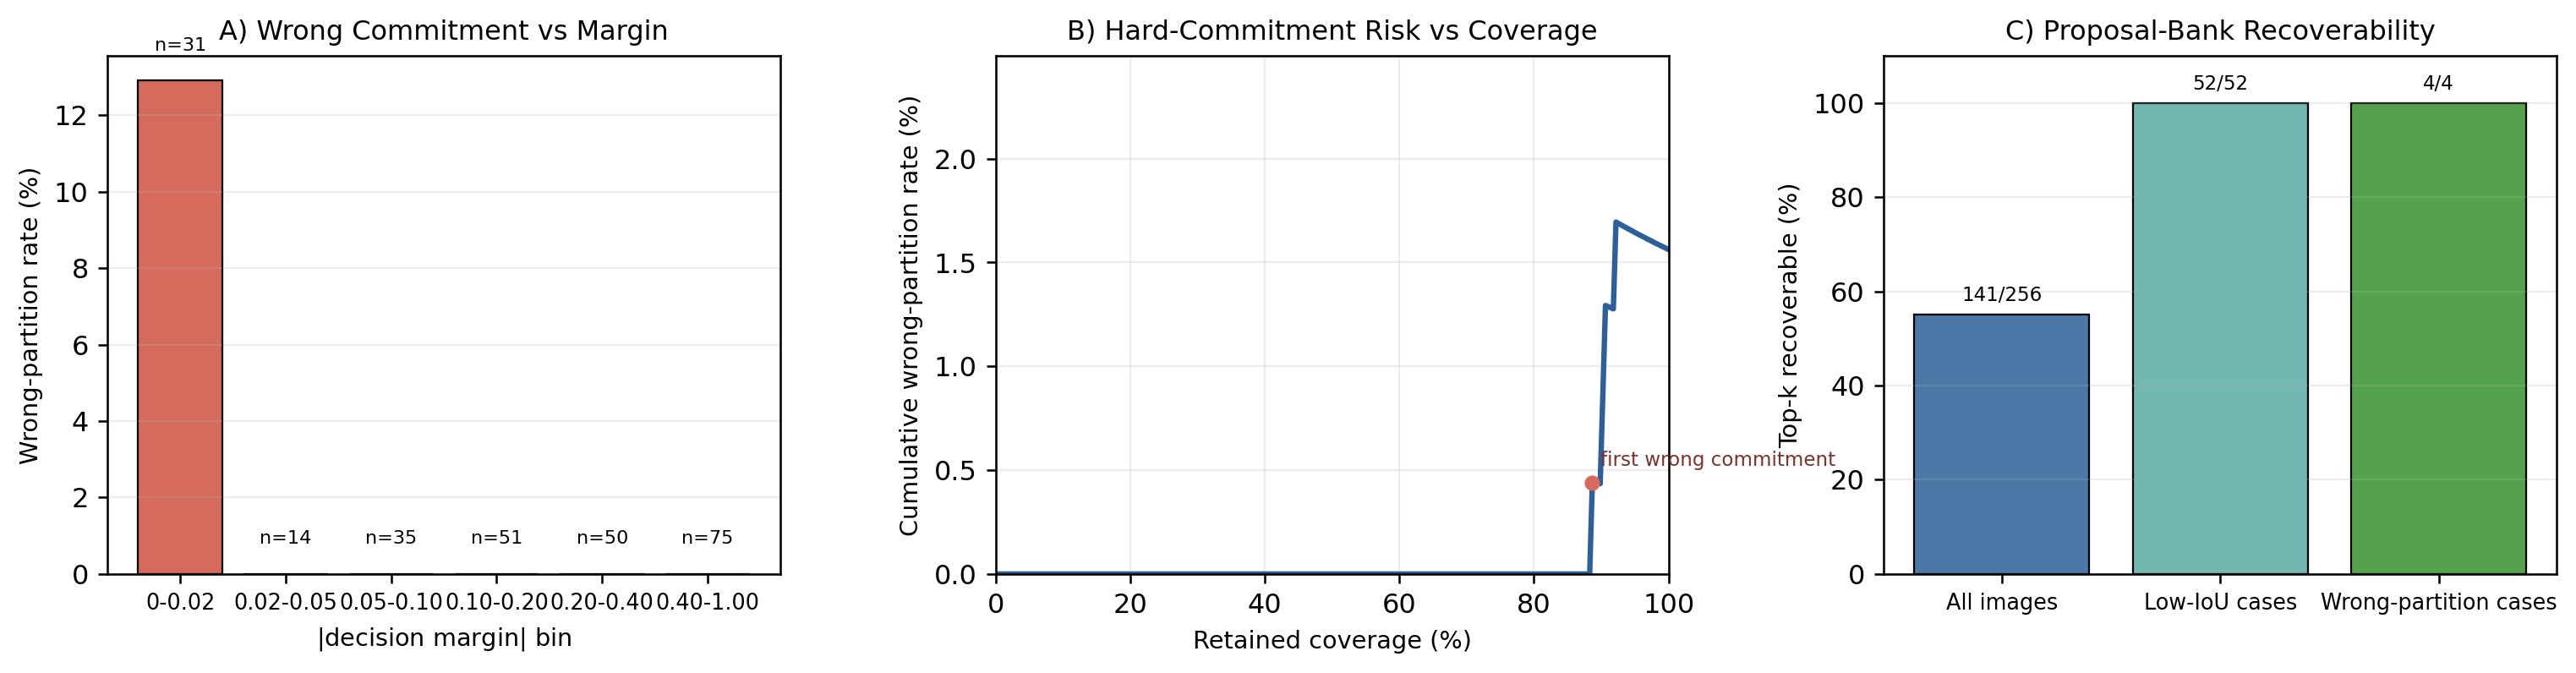
\includegraphics[width=0.92\textwidth]{figures/fig_ambiguity_commitment_full256.png}
    \caption{RWTD ambiguity-to-failure diagnostics on the full-256 audit. Wrong-partition cases concentrate in the lowest-margin regime, and top-$k$ recoverability remains high exactly where the final decision layer is most brittle.}
    \label{fig:ambiguity_commitment}
\end{figure*}

\paragraph{How to read the oracle gap.} The bank upper bound is not a deployable method: it assumes access to the ground-truth partition when choosing among proposals, merged components, and rescue candidates. Its role is diagnostic. On RWTD, the gap between the deployed system and that bound shows that the frozen bank already contains more usable texture evidence than the current decision layer recovers. The learned single-selector baseline narrows only part of that gap, which is why RWTD still needs structured commitment above fragmented proposals.

\begin{table*}[t]
\centering
\small
\begin{tabularx}{\textwidth}{@{}Xccccccc@{}}
\toprule
Setting & Resc. & Off-succ. & Hurt-any & Wrong & Unsafe & Mean $\Delta$IoU & Top-$k$ recov. \\
\midrule
Baseline decision rule & 21 & 61.9\% & 38.1\% & 4 & 6 & +0.2247 & 141/256 \\
\bottomrule
\end{tabularx}
\caption{RWTD full-256 failure-audit summary for the deployed decision rule. The remaining weakness is ambiguity-aware commitment rather than proposal-bank absence.}
\label{tab:rwtd_audit}
\end{table*}

\begin{table*}[t]
\centering
\scriptsize
\begin{tabularx}{\textwidth}{@{}Xcc@{}}
\toprule
Dense rescue proposal source (frozen) & Full-256 mIoU / ARI & Common-253 mIoU / ARI \\
\midrule
Released dense bank & 0.4611 / 0.6966 & 0.4645 / 0.7013 \\
SAM2.1-large source swap & 0.5003 / 0.7048 & 0.5005 / 0.7106 \\
\bottomrule
\end{tabularx}
\caption{Frozen proposal-source transfer stress test. Consolidation weights and thresholds remain fixed; only the rescue proposal bank changes. This is evidence for modularity of the decision layer, not a standalone benchmark claim.}
\label{tab:proposal_swap}
\end{table*}

\begin{table*}[t]
\centering
\scriptsize
\setlength{\tabcolsep}{5pt}
\renewcommand{\arraystretch}{0.98}
\begin{tabularx}{\textwidth}{@{}p{0.22\textwidth}p{0.17\textwidth}cc@{}}
\toprule
Comparison & Paired units & $\Delta$ mIoU (95\% interval) & $\Delta$ ARI (95\% interval) \\
\midrule
RWTD common-253, \sys{} $-$ TextureSAM & 426 overlapped GT instances & $+0.0405$ [$0.0031$, $0.0764$] & $+0.0995$ [$0.0721$, $0.1270$] \\
STLD all-200, \sys{} $-$ TextureSAM & 200 images & $+0.2028$ [$0.1555$, $0.2486$] & $+0.0400$ [$0.0049$, $0.0754$] \\
STLD common-182, \sys{} $-$ TextureSAM & 182 images & $+0.2055$ [$0.1558$, $0.2518$] & $+0.0265$ [$-0.0097$, $0.0605$] \\
\bottomrule
\end{tabularx}
\caption{Paired interval support for the matched comparisons. RWTD uses the official overlap-instance view because the published no-aggregation metric averages GT instances overlapped by each method rather than simple per-image means. STLD intervals are paired per-image bootstraps under the direct-foreground evaluator.}
\label{tab:bootstrap_support}
\end{table*}

\begin{table*}[t]
\centering
\small
\begin{tabularx}{\textwidth}{@{}p{0.30\textwidth}X@{}}
\toprule
Item & Value \\
\midrule
External training data & PTD only for RWTD, the ADE20K-selected complement, the ControlNet bridge complement, and the appendix CAID route; Brodatz-native synthetic supervision for STLD \\
Encoder training data & 80{,}000 train / 20{,}000 val images per synthetic source \\
RWTD benchmark usage & Evaluation only; no RWTD-label training or hyperparameter search \\
Proposal source & Frozen SAM-style automatic masks \\
RWTD / STLD deployed model & Swin-Base masked-region encoder with learned merge/core/repair modules \\
ADE20K / ControlNet / CAID appendix deployed model & PTD-trained \texttt{small\_pre\_ring\_hi} Stage-A bundle \\
Primary evaluator & Official upstream no-aggregation evaluator on RWTD; route-matched evaluators elsewhere \\
Comparator family & Raw SAM2.1-small plus reproduced/public TextureSAM checkpoints \\
\bottomrule
\end{tabularx}
\caption{Compact reproducibility summary for the manuscript scope.}
\label{tab:compact_repro}
\end{table*}


\section{STLD Supporting Oracle Analysis}
\label{app:stld_support}

STLD plays a different supporting role. The oracle analysis still shows extra headroom in the bank, but the learned top-1 selector is already close to the full system on the common-182 subset. In practice, many STLD images contain a coherent singleton answer, so the main remaining gain is modest coherence cleanup rather than large-scale fragment commitment.

\begin{table*}[t]
\centering
\scriptsize
\begin{tabularx}{\textwidth}{@{}XccccX@{}}
\toprule
Dataset / subset & Selector mIoU & Selector ARI & Final mIoU & Final ARI & Reading \\
\midrule
RWTD common-253 & 0.4512 & 0.5601 & 0.4645 & 0.7013 & Large ARI gap: fragmented natural scenes still need structured commitment above the frozen bank. \\
STLD common-182 & 0.7196 & 0.7731 & 0.7195 & 0.7791 & Near-parity: a coherent singleton answer often already exists, so commitment adds only a small coherence gain. \\
\bottomrule
\end{tabularx}
\caption{Cross-dataset contrast between learned top-1 selection and full proposal-space commitment. RWTD and STLD use different evaluators, so the point is not absolute scale but the different role played by singleton selection on the two routes.}
\label{tab:stld_selector_contrast}
\end{table*}


\begin{figure*}[t]
    \centering
    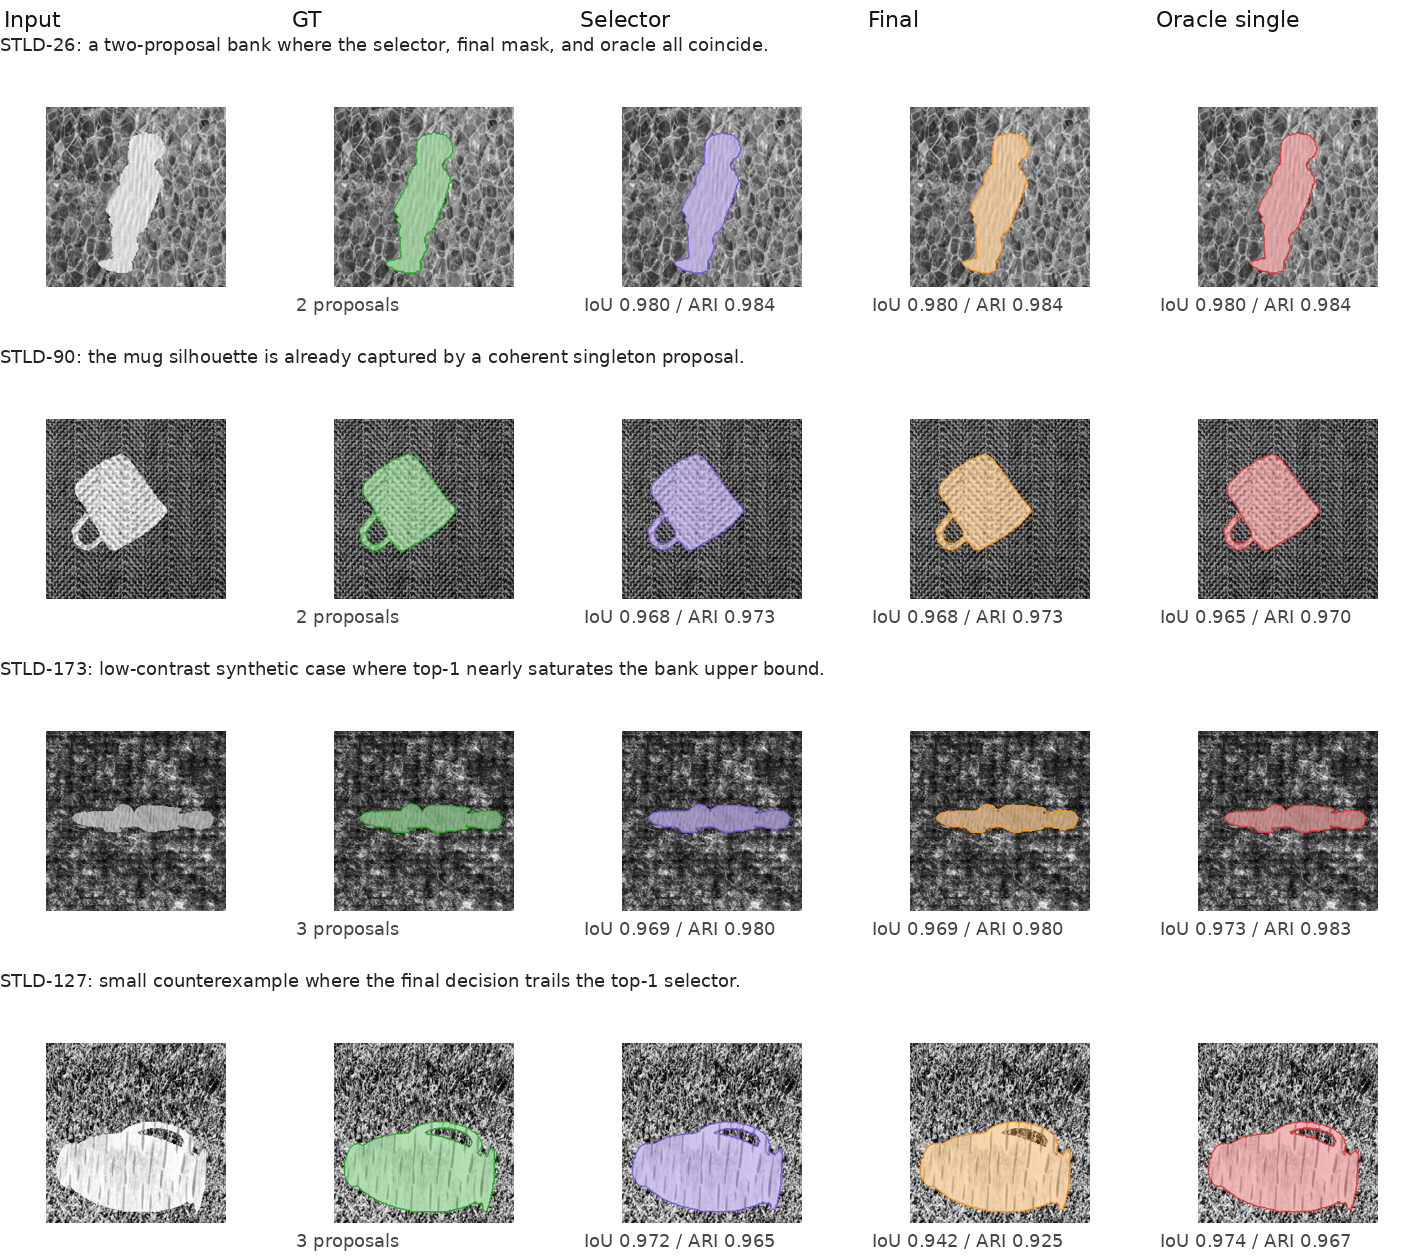
\includegraphics[width=0.96\textwidth]{figures/fig_stld_case_gallery.png}
    \caption{Representative STLD cases. Most examples already have a coherent singleton proposal, so the learned selector, final deployment, and single-proposal oracle are nearly indistinguishable. The last row shows a useful counterexample where the selector slightly outruns the final decision.}
    \label{fig:stld_case_gallery}
\end{figure*}

\begin{table*}[t]
\centering
\scriptsize
\setlength{\tabcolsep}{5pt}
\renewcommand{\arraystretch}{0.98}
\begin{tabular}{@{}lcccc@{}}
\toprule
STLD method & All-200 mIoU & All-200 ARI & Common-182 mIoU & Common-182 ARI \\
\midrule
Proposal route final & 0.6705 & 0.7249 & 0.7195 & 0.7791 \\
Learned single selector & 0.6548 & 0.7036 & 0.7196 & 0.7731 \\
Single frozen-proposal oracle & 0.7375 & 0.7684 & 0.8105 & 0.8444 \\
Compatible-component oracle & 0.3950 & 0.3598 & 0.4341 & 0.3953 \\
Top-$k$ union oracle & 0.1257 & 0.0289 & 0.1381 & 0.0317 \\
Bank upper bound & 0.7574 & 0.7962 & 0.8149 & 0.8574 \\
\bottomrule
\end{tabular}
\caption{Supporting STLD oracle analysis under the direct-foreground evaluator. The learned top-1 selector already recovers much of the overlap on STLD, but the full proposal-route readout remains slightly stronger on coherence and still trails the bank oracles.}
\label{tab:stld_oracles}
\end{table*}


\section{Supporting Routes}
\label{app:route_secondary}

The remaining routes stay secondary by design. The ControlNet-stitched bridge benchmark preserves exact supervision while introducing more naturalistic transitions than hard mosaics, but this paper does not claim a causal bridge-training benefit. CAID is kept only as a breadth check under domain shift.

\subsection{ControlNet Bridge Examples}
\label{app:bridge_secondary}

\begin{figure*}[t]
    \centering
    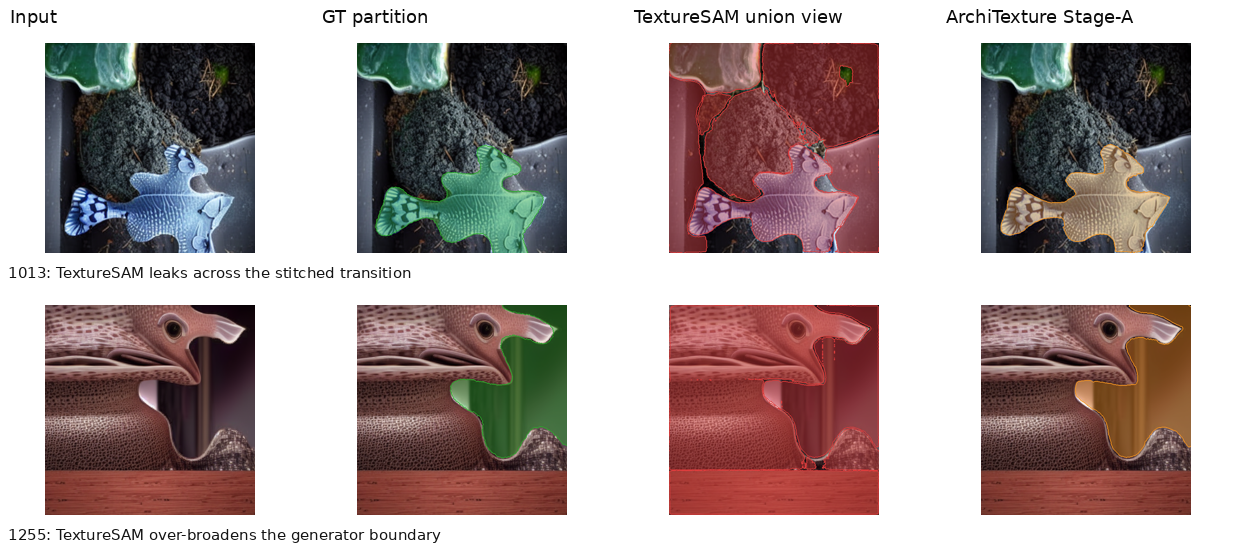
\includegraphics[width=0.92\textwidth]{figures/fig_controlnet_bridge_examples.png}
    \caption{ControlNet-stitched bridge examples. The proposal-union view often leaks across the stitched transition or over-broadens the generator boundary, which explains why overlap can look reasonable while ARI remains fragile. The Stage-A route is more conservative, but we keep this benchmark in the appendix because the paper does not establish a causal bridge-training advantage.}
    \label{fig:controlnet_bridge_app}
\end{figure*}

\begin{table*}[t]
\centering
\scriptsize
\begin{tabularx}{\textwidth}{@{}Xlcc@{}}
\toprule
Method & Subset / coverage & Direct mIoU / ARI & Invariant mIoU / ARI \\
\midrule
TextureSAM public checkpoint rerun & all-1742, 1739/1742 & 0.4212 / 0.6446 & 0.6425 / 0.5510 \\
Proposal route Stage-A & all-1742, 1742/1742 & 0.4993 / 0.6039 & 0.6803 / 0.6039 \\
TextureSAM public checkpoint rerun & common-1739 & 0.4219 / 0.6457 & 0.6436 / 0.5519 \\
Proposal route Stage-A & common-1739 & 0.4993 / 0.6039 & 0.6803 / 0.6039 \\
\bottomrule
\end{tabularx}
\caption{ControlNet-stitched synthetic complement. This route broadens the synthetic side beyond the classical STLD benchmark by preserving exact labels while using more naturalistic stitched transitions. The main text emphasizes the invariant view; this appendix table retains the direct and matched-subset views together.}
\label{tab:controlnet_secondary}
\end{table*}


\subsection{CAID Breadth Check}
\label{app:caid_secondary}

\begin{figure*}[t]
    \centering
    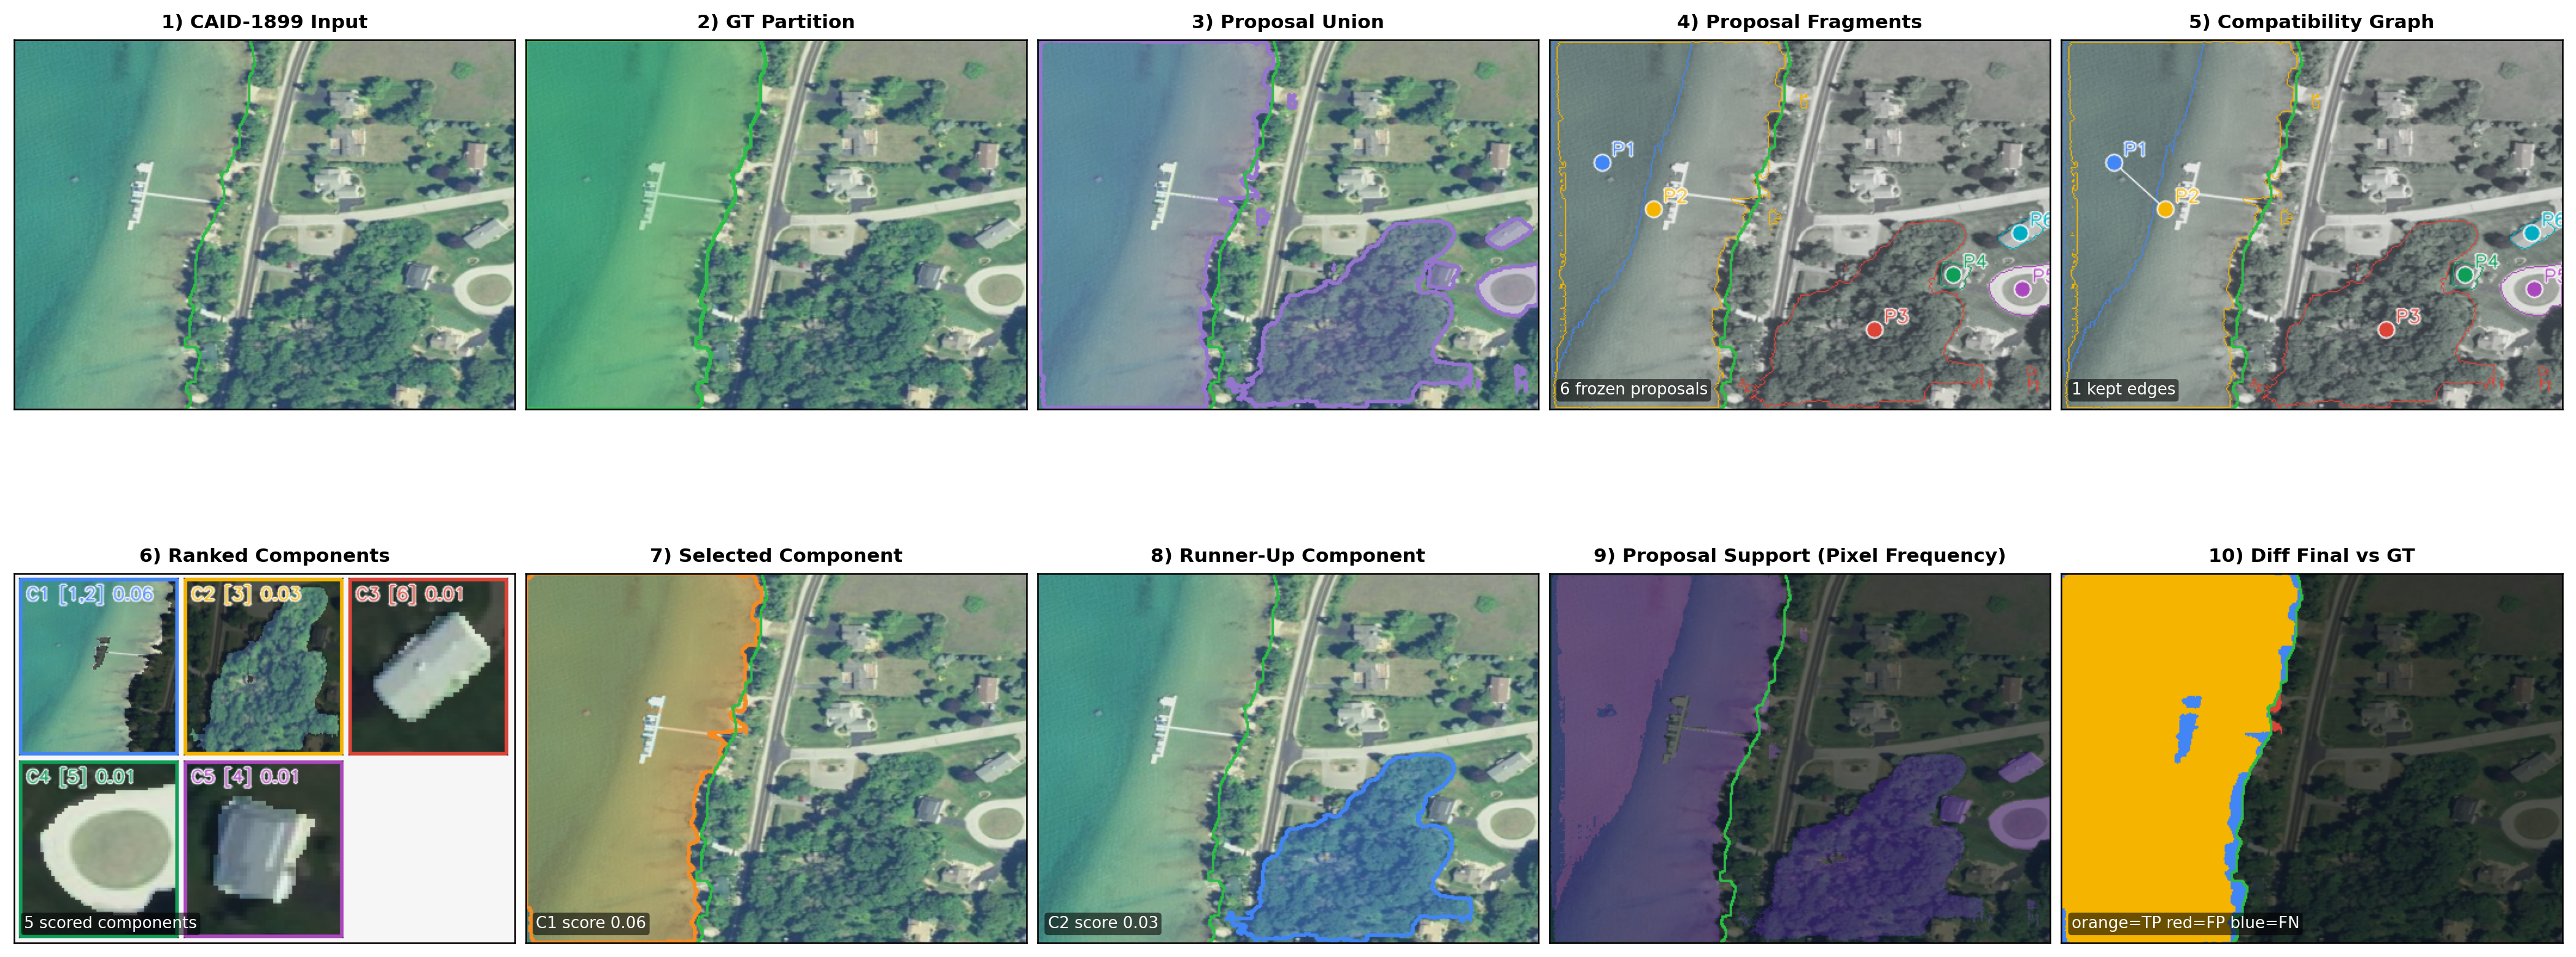
\includegraphics[width=0.98\textwidth]{figures/fig_caid_audit.png}
    \caption{CAID breadth-check example. The same frozen-bank consolidation logic remains useful under shoreline structure, but this route is not central to the paper's texture claim and is reported only as an appendix-side generalization check.}
    \label{fig:caid_app}
\end{figure*}

\begin{table*}[t]
\centering
\scriptsize
\begin{tabularx}{\textwidth}{@{}Xlc@{}}
\toprule
Method & Subset / coverage & Invariant mIoU / ARI \\
\midrule
TextureSAM public checkpoint rerun & all-3104, 3063/3104 & 0.6691 / 0.5080 \\
Proposal route Stage-A & all-3104, 3104/3104 & 0.6677 / 0.5745 \\
TextureSAM public checkpoint rerun & common-3063 & 0.6780 / 0.5148 \\
Proposal route Stage-A & common-3063 & 0.6677 / 0.5745 \\
\bottomrule
\end{tabularx}
\caption{CAID appendix real-world complement under the partition-invariant evaluator. CAID is retained separately because its exact shoreline masks and large contiguous land/water partitions are useful but narrower than the paper's central natural/synthetic texture settings.}
\label{tab:caid_secondary}
\end{table*}



\end{document}
